%%
%% This is file `sample-sigconf.tex',
%% generated with the docstrip utility.
%%
%% The original source files were:
%%
%% samples.dtx  (with options: `all,proceedings,bibtex,sigconf')
%% 
%% IMPORTANT NOTICE:
%% 
%% For the copyright see the source file.
%% 
%% Any modified versions of this file must be renamed
%% with new filenames distinct from sample-sigconf.tex.
%% 
%% For distribution of the original source see the terms
%% for copying and modification in the file samples.dtx.
%% 
%% This generated file may be distributed as long as the
%% original source files, as listed above, are part of the
%% same distribution. (The sources need not necessarily be
%% in the same archive or directory.)
%%
%%
%% Commands for TeXCount
%TC:macro \cite [option:text,text]
%TC:macro \citep [option:text,text]
%TC:macro \citet [option:text,text]
%TC:envir table 0 1
%TC:envir table* 0 1
%TC:envir tabular [ignore] word
%TC:envir displaymath 0 word
%TC:envir math 0 word
%TC:envir comment 0 0
%%
%% The first command in your LaTeX source must be the \documentclass
%% command.
%%
%% For submission and review of your manuscript please change the
%% command to \documentclass[manuscript, screen, review]{acmart}.
%%
%% When submitting camera ready or to TAPS, please change the command
%% to \documentclass[sigconf]{acmart} or whichever template is required
%% for your publication.
%%
%%
\documentclass[sigplan]{acmart}

\usepackage[utf8]{inputenc}
\usepackage[T1]{fontenc}
\usepackage{amsmath}
\let\Bbbk\relax 
\usepackage{amssymb}
\usepackage{amsfonts}
\usepackage{algorithm,algpseudocode}
\usepackage{graphicx}
\usepackage{booktabs}
\usepackage{hyperref}
\usepackage{xcolor}
\usepackage{tikz}
\usepackage{caption}
\usepackage{subcaption}
\usepackage{listings}
\usepackage{multirow}
\usepackage{url}

% Hyperref setup
\hypersetup{
    colorlinks=true,
    linkcolor=blue,
    filecolor=magenta,      
    urlcolor=cyan,
    citecolor=blue
}


\usepackage{tabularx} % put this in your preamble
\usepackage{graphicx}
% \usepackage[tt=false, type1=true]{libertine}
% \usepackage{newtxtext,newtxmath}
%\usepackage{amssymb}
% \usepackage[varqu]{zi4}
\usepackage[T1]{fontenc}
\usepackage{enumitem}
%\usepackage{amsmath}
\usepackage{soul}
\usepackage{url}
\usepackage{subcaption}
\usepackage{array} % for better column formatting
\usepackage{booktabs} % for nicer tables

\usepackage{xspace}
\usepackage{xcolor}
\usepackage{wrapfig} 
\usepackage{caption} % for captions in minipages
\usepackage{booktabs} % for tables
\usepackage{tikz}

\usepackage{listings}
\usepackage{xcolor}

% \lstset{
%   basicstyle=\ttfamily\footnotesize,
%   breaklines=true,
%   columns=fullflexible,
%   keepspaces=true
% }
\usetikzlibrary{positioning,arrows.meta,calc}
\newcommand{\rn}[1]{{\textcolor{red}{RN: #1}}}
\newcommand{\fillin}[1]{{\textcolor{red}{#1}}}

\newcommand{\mw}[1]{{\textcolor{cyan}{MW: #1}}}
\newcommand{\sn}[1]{{\textcolor{blue}{[SN: #1]}}}
\newcommand{\kh}[1]{\textcolor{magenta}{KH: #1}}


\newcommand{\para}[1]{\medskip\noindent\textbf{#1}}
\newcommand{\paraf}[1]{\noindent\textbf{#1}}
\newenvironment{parafont}{\fontfamily{ptm}\selectfont}{}


\newcommand{\Para}[1]{\vspace{2pt}\noindent\begin{parafont}\textbf{\textit{#1}}\end{parafont}}
\newcommand{\TheThing}{{\sc Glenfinnan}\xspace} 
%%
%% \BibTeX command to typeset BibTeX logo in the docs
\AtBeginDocument{%
  \providecommand\BibTeX{{%
    Bib\TeX}}}

%% Rights management information.  This information is sent to you
%% when you complete the rights form.  These commands have SAMPLE
%% values in them; it is your responsibility as an author to replace
%% the commands and values with those provided to you when you
%% complete the rights form.
%\setcopyright{acmlicensed}
%\copyrightyear{2018}
%\acmYear{2018}
%\acmDOI{XXXXXXX.XXXXXXX}
%% These commands are for a PROCEEDINGS abstract or paper.
%\acmConference[EuroSys '27]{Make sure to enter the correct
%  conference title from your rights confirmation email}{June 03--05,
%  2018}{Woodstock, NY}
%%
%%  Uncomment \acmBooktitle if the title of the proceedings is different
%%  from ``Proceedings of ...''!
%%
%%\acmBooktitle{Woodstock '18: ACM Symposium on Neural Gaze Detection,
%%  June 03--05, 2018, Woodstock, NY}
%\acmISBN{978-1-4503-XXXX-X/2018/06}


%%
%% Submission ID.
%% Use this when submitting an article to a sponsored event. You'll
%% receive a unique submission ID from the organizers
%% of the event, and this ID should be used as the parameter to this command.
%%\acmSubmissionID{123-A56-BU3}

%%
%% For managing citations, it is recommended to use bibliography
%% files in BibTeX format.
%%
%% You can then either use BibTeX with the ACM-Reference-Format style,
%% or BibLaTeX with the acmnumeric or acmauthoryear sytles, that include
%% support for advanced citation of software artefact from the
%% biblatex-software package, also separately available on CTAN.
%%
%% Look at the sample-*-biblatex.tex files for templates showcasing
%% the biblatex styles.
%%

%%
%% The majority of ACM publications use numbered citations and
%% references.  The command \citestyle{authoryear} switches to the
%% "author year" style.
%%
%% If you are preparing content for an event
%% sponsored by ACM SIGGRAPH, you must use the "author year" style of
%% citations and references.
%% Uncommenting
%% the next command will enable that style.
%%\citestyle{acmauthoryear}

\newcommand{\tightcaption}[1]{\vspace{-7pt}\caption{{\bf \small #1}}
\vspace{-8pt}
}

%%
%% end of the preamble, start of the body of the document source.
\setcopyright{none}
\settopmatter{printacmref=false}
\renewcommand\footnotetextcopyrightpermission[1]{} 
\pagestyle{plain}
%\renewcommand\footnotetextcopyrightpermission[1]{}
\begin{document}

%%
%% The "title" command has an optional parameter,
%% allowing the author to define a "short title" to be used in page headers.
% \title{\sys: Profile-Guided Speculation for Fast Web Agents}
\title{\sys: Speculative Execution for Fast and Efficient Web Agents}

%%
%% The "author" command and its associated commands are used to define
%% the authors and their affiliations.
%% Of note is the shared affiliation of the first two authors, and the
%% "authornote" and "authornotemark" commands
%% used to denote shared contribution to the research.
\author{Mike Wong}
\affiliation{%
  \institution{Princeton University}
    \city{Princeton}
  \country{USA}
}
\author{Kevin Hsieh}
\affiliation{%
  \institution{Microsoft Research}
    \city{Seattle}
  \country{USA}
}
\author{Suman Nath}
\affiliation{%
  \institution{Microsoft Research}
    \city{Seattle}
  \country{USA}
}
\author{Ravi Netravali}
\affiliation{%
  \institution{Princeton University}
   \city{Princeton}
  \country{USA}
}
% \email{webmaster@marysville-ohio.com}



%%
%% By default, the full list of authors will be used in the page
%% headers. Often, this list is too long, and will overlap
%% other information printed in the page headers. This command allows
%% the author to define a more concise list
%% of authors' names for this purpose.
\renewcommand{\shortauthors}{M. Wong et al.}
\newcommand{\sys}{{Skim}\xspace} 
% \newcommand{\sys}{{Skim}\xspace} 

%%
%% The abstract is a short summary of the work to be presented in the
%% article.


\addtolength{\textheight}{-0.25in}



% \begin{abstract}
% Skim is a speculative execution framework for web agents that
% exploits the predictable structure of purpose-built websites.
% Today's web-agent expense is not intrinsic to the tasks but a
% property of how agents are composed: frontier-model inference,
% browser rendering, and ReAct-style planning are applied to every
% step of every task regardless of complexity. Skim's key
% observation is that websites enforce stable URL patterns, answer
% formats, and task-to-trajectory mappings across queries of the
% same type, so most queries can bypass these heavyweight
% components entirely. An offline profiler captures these patterns
% once per site. At runtime, Skim matches each query to a
% template, synthesizes the destination URL, and extracts the
% answer with a small model. A lightweight verifier gates each
% fast-path output against the query and schema; rare
% misspeculations cascade to the full agent, warm-started by the
% fast path's final URL to preserve upstream trajectory progress.
% Across standard web-agent benchmarks paired with three backbone
% agents (WebVoyager, AgentOccam, BrowserUse), Skim reduces median
% per-task cost by 1.9$\times$ and latency by 33.4\% with no
% accuracy loss.
% \end{abstract}

\begin{abstract}

% Web agents have shown powerful capabilities to autonomously complete tasks by directly browsing the live web, but their inflated per-task costs and latencies have limited their practical adoption. We argue these overheads are not intrinsic to the task at hand, and instead stem from their composition. Specifically, websites are purpose-built around the queries users bring to them, exposing intrinsic structure in page organization and stable mappings from task types to trajectories that together unlock substantial savings opportunities -- savings that today's agents miss by defaulting to frontier models, browsers, and sequential ReAct execution at every step regardless of what is actually required. We present \sys, a speculative execution framework for web agents that pairs offline site-structure profiling with online selection and validation of speculative fast paths. To ensure high accuracy despite the massive space of per-page actions (and thus trajectories per query), \sys reduces runtime selection to a lookup against a per-site catalog of task-type templates and answer formats, exploiting the fact that both are stable across queries of the same task type. A small judge model gates each fast-path output against the query and schema, falling back to the full agent on rare misspeculations warm-started by the fast path's final URL to exploit upstream trajectory overlaps. Across popular benchmarks and web agents, \sys reduces median per-task cost by 1.9$\times$ and latency by 33.4\% while preserving accuracy. 

Skim is a speculative execution framework for web agents that exploits the predictable structure of purpose-built websites. Today's web-agent expense is not intrinsic to the tasks but a property of how agents are composed: frontier-model inference, browser rendering, and ReAct-style planning are applied to every step of every task regardless of complexity. Skim's key observation is that websites enforce stable URL patterns, answer formats, and task-to-trajectory mappings across queries of the same type, so most queries can bypass these heavyweight components entirely. An offline profiler captures these patterns once per site. At runtime, Skim matches each query to a template, synthesizes the destination URL, and extracts the answer with a small model. A lightweight verifier gates each fast-path output against the query and schema; rare misspeculations cascade to the full agent, warm-started by the fast path's final URL to preserve upstream trajectory progress. Across standard web-agent benchmarks paired with three backboneagents (WebVoyager, AgentOccam, BrowserUse), Skim reduces median per-task cost by 1.9x and latency by 33.4\% with no accuracy loss.

\end{abstract}


%%
%% Keywords. The author(s) should pick words that accurately describe
%% the work being presented. Separate the keywords with commas.
\keywords{}

\received{20 February 2007}
\received[revised]{12 March 2009}
\received[accepted]{5 June 2009}

%%
%% This command processes the author and affiliation and title
%% information and builds the first part of the formatted document.
\maketitle


\newcommand{\todo}[1]{\textcolor{red}{[TODO: #1]}}
\newcommand{\note}[1]{\textcolor{blue}{\textit{Note: #1}}}
\newcommand{\figplaceholder}[2]{%
  \begin{center}
  \fbox{\parbox{0.85\linewidth}{\centering\vspace{1em}\textbf{Figure \ref*{#1}: #2}\\[0.5em]\textcolor{gray}{[placeholder]}\vspace{1em}}}
  \end{center}
}


% \input{outline}
\section{Introduction}

\begin{sloppypar}
Web agents, or LLM-based systems that complete tasks by directly browsing and interacting with live websites, are increasingly deployed in retrieval-augmented assistants, deep-research tools, and enterprise automation pipelines. Agents such as WebVoyager~\cite{webvoyager}, AgentOccam~\cite{agentoccam}, and BrowserUse~\cite{browseruse} now underpin a fast-growing class of products that resolve queries no static corpus can answer: navigating to authenticated pages, completing multi-step lookups across catalogs, and extracting structured information from sites the user does not need to visit themselves. This capability far exceeds what stateless retrieval pipelines (e.g., Perplexity, ChatGPT browsing) achieve by querying search indices and synthesizing from snippets -- they cannot maintain authenticated state, complete multi-step trajectories, or reach content beyond search coverage -- but it comes at substantial overhead: per-task latencies run 30-120 secs and API costs run \$0.20-0.50, 1-2 orders of magnitude more than stateless retrieval. %At deployment scale, these per-task costs compound into operational expenses that bound adoption.
\end{sloppypar}

The high overheads of web agents trace to three off-the-shelf components, each designed for problems broader than the web tasks they typically execute. Frontier LLMs are trained for long-context multi-hop reasoning; browsers are engineered for arbitrary and secure human interaction with any web page; ReAct is a general decision-making framework for agents in unconstrained environments with sparse feedback. Each component is highly capable, but fails to exploit the structural regularities that the web exhibits. The first such property is \emph{step heterogeneity}. Most steps in a typical web agent trajectory are mechanical (fetch a known URL, locate a labeled field on a page, click a stable navigation element) and do not require frontier reasoning or full browser execution. The second is \emph{task-driven structure}. Sites are purpose-built around the queries users bring to them, so URL templates, page layouts, and answer formats are stable across queries of the same type. For instance, the navigation pattern that resolves one arXiv lookup resolves the next, with only query-specific identifiers changing. Together, these properties imply that many steps can run on cheaper components, and many can be skipped entirely by following trajectories the site has already revealed.

Our analysis of popular web agent tasks confirms that the opportunity is substantial (\S\ref{sec:opp}). Hand-engineered programs that exploit website structure by using trajectory knowledge to fetch via direct URLs, prune to answer-bearing content, and extract with cheaper models can run 66.7-94.9\% faster and 17.7-100.7$\times$ cheaper than the off-the-shelf ReAct agent without any accuracy loss. However, automating this strategy in practice is difficult; naively substituting these cheaper techniques inside an off-the-shelf ReAct loop drops average task success by 60\%. The issue is that cheap models struggle to choose the right action from the hundreds of interactive elements on a typical page, and direct-URL fetching requires knowing in advance precisely which page will contain the answer for a given query (\S\ref{sec:chal}). Worse, errors compound across a trajectory, so a single wrong step can invalidate everything downstream. The core question is thus how to identify, when a query arrives, which shortcuts preserve accuracy for \emph{that} query -- a question made difficult by the heterogeneity of tasks, the variation across pages in a site, and the per-step diversity in resource needs.

%Our analysis of popular web agent tasks confirms the opportunity is substantial (\S\ref{sec:motivation:handtune}). Hand-engineered programs that exploit website structure by using trajectory knowledge to fetch via direct URLs, prune to answer-bearing content, and extract with cheaper models can drop per-task cost by X$\times$ and latency by Y\% without accuracy loss. However, realizing this strategy in practice is difficult --  naively substituting these cheaper techniques inside an off-the-shelf ReAct loop drops task success by Y\%, because even a single wrong step can compound across the trajectory and invalidate the result (\S\ref{sec:motivation}) \mw{Do we want to mention the other core reasons for failure? Namely that the action space is too large for small models, direct fetching requires a priori knowledge of trajectories, etc. }. The core question is thus how to identify, when a query arrives, which shortcuts preserve accuracy for \emph{this} query? Tasks vary in objects and objectives, sites vary internally across page types, and the minimum-sufficient resource varies per step within a single trajectory, all of which make this identification difficult to do cheaply and reliably.

To address these challenges, we present \textbf{\sys}, a drop-in acceleration framework for existing web agents. The key insight underlying \sys{} is that web sites are \emph{predictable enough to precompute} navigation paths offline, and \emph{structured enough to check} answer correctness online. Sites change rarely relative to query rates, so trajectory patterns characterized once per task type remain valid across many future queries. Further, since sites impose stable formats on task result pages (e.g., search results), a fast path's output can be easily validated against both the query and the expected schema, without invoking the expensive agent. Building on this, \sys{} profiles each reachable site offline, recording for each task type both the shortcuts that apply (URL patterns reaching its result pages) and what correct outputs look like (the answer schemas of those pages). At runtime, when a query arrives, \sys{} consults the profile and, if covered, speculatively attempts a fast path via direct URL fetch and cheap model processing, accepting the result only when a small judge model deems it consistent with the query and the recorded schema. Upon failure, \sys{} falls back to the full ReAct agent, warm-started at the URL the fast path reached -- since trajectories share predictable prefixes, even failed shortcuts reduce the work that the agent must redo.




%To address these challenges, we present \textbf{\sys}, a drop-in acceleration framework for existing web agents. The key insight underlying \sys is that web sites are cheap to \emph{profile} offline and cheap to \emph{verify} online. Sites change rarely relative to query rates, so an infrequent investment in modeling each site's recurring trajectories amortizes across many future queries. Moreover, since answer formats are determined by site purpose, a correct output can be recognized without re-running the full agent. Building on this, \sys{} profiles each reachable site offline, recording URL templates and answer schemas for the task types it encounters. At runtime, when a query arrives, \sys{} consults the profile and, if covered, attempts a fast path that fetches the candidate URL, extracts with a non-frontier model, and validates the output against the recorded schema. Upon failures, \sys{} falls back to the full ReAct agent, warm-started at the URL the fast path already reached, so navigational progress carries over rather than being discarded.


We evaluate \sys on two representative benchmarks (WebVoyager, WebShop) across three popular ReAct-based web agents (BrowserUse, AgentOccam, WebVoyager). We consider two deployment modes that exploit the same underlying mechanism. In \emph{accelerate} mode, \sys lowers median per-task cost by 1.9$\times$ and latency by 33.4\% while preserving accuracy. In \emph{aggregate} mode, \sys reinvests the saved compute budget into multiple trials that explore different trajectories with verifier-selected outputs. Within the single-trial baseline's cost budget, this lifts end-to-end accuracy by up to 16.7 percentage points (4.2 pp with majority vote).



\begin{figure}[t]
    \centering
    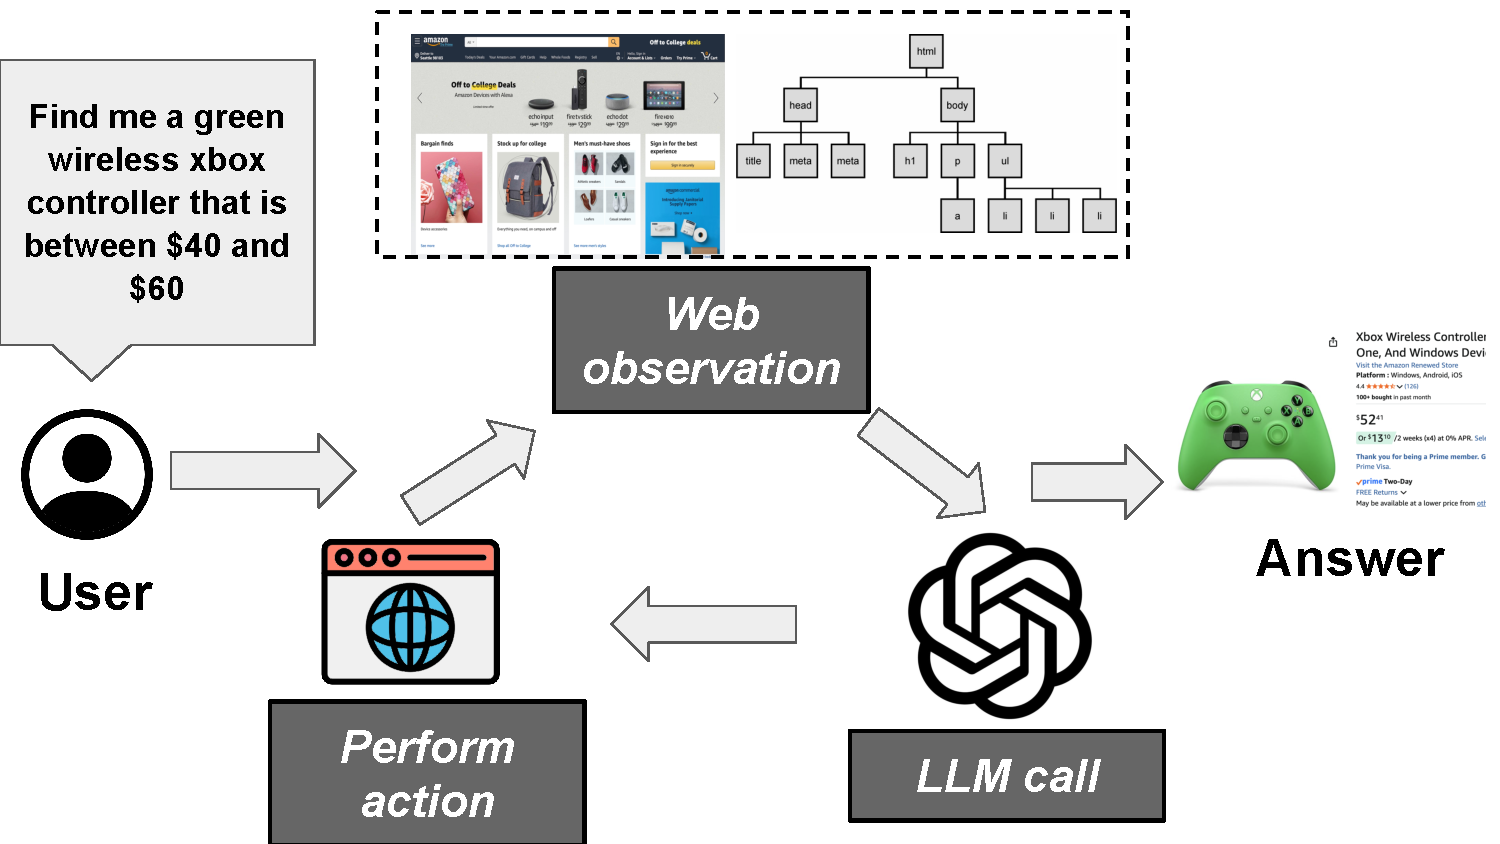
\includegraphics[width=0.8\columnwidth]{figures/5-4-2026/react-workflow.pdf}
    \tightcaption{Workflow of a representative ReAct-based web agent.
    The agent loops through render, observe, reason, and act steps
    until task completion.}
    \label{fig:react-workflow}
\end{figure}



\section{Background and Motivation}
\label{sec:background}

Web agents incur substantial overheads not intrinsic to their tasks. We examine where these overheads come from, identify the structural properties that make them avoidable, and characterize the challenges of automating their removal.





\begin{figure}[t]
    \centering
    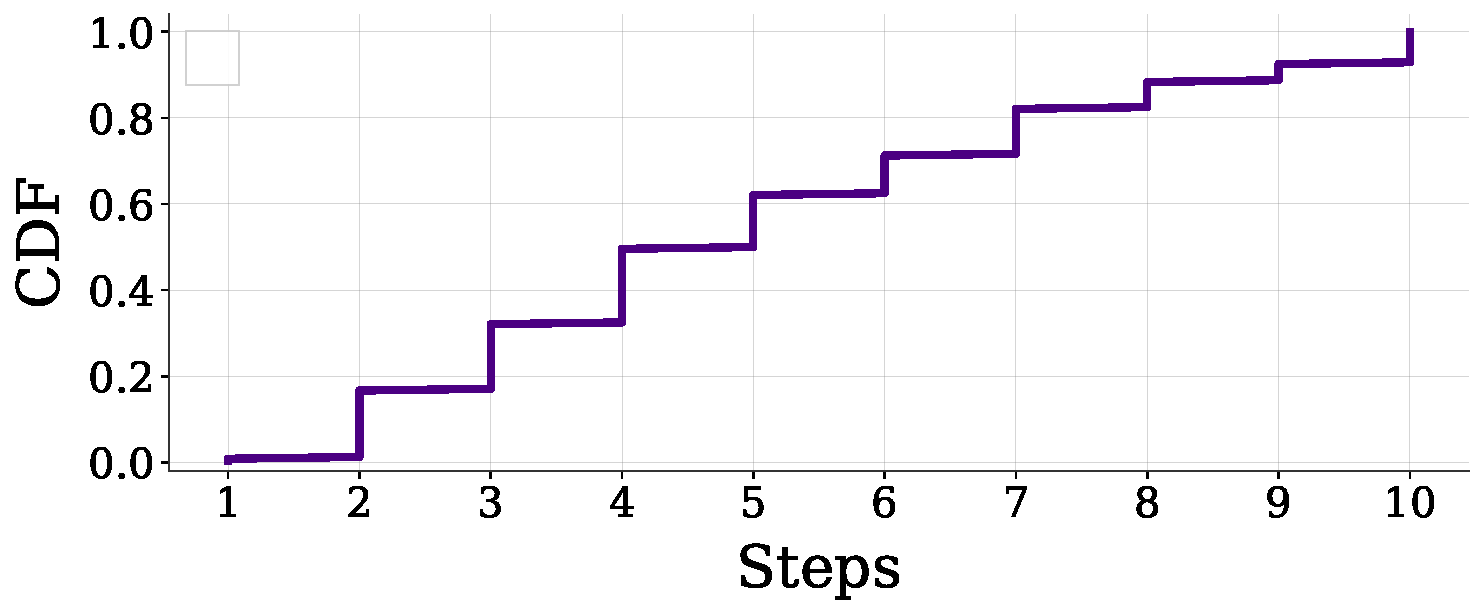
\includegraphics[width=0.8\columnwidth]{figures/steps_cdf.pdf}
    \tightcaption{Distribution of number of ReAct steps needed for agents to converge to an answer.}
    \label{fig:steps}
\end{figure}

\begin{figure}[t]
    \centering
    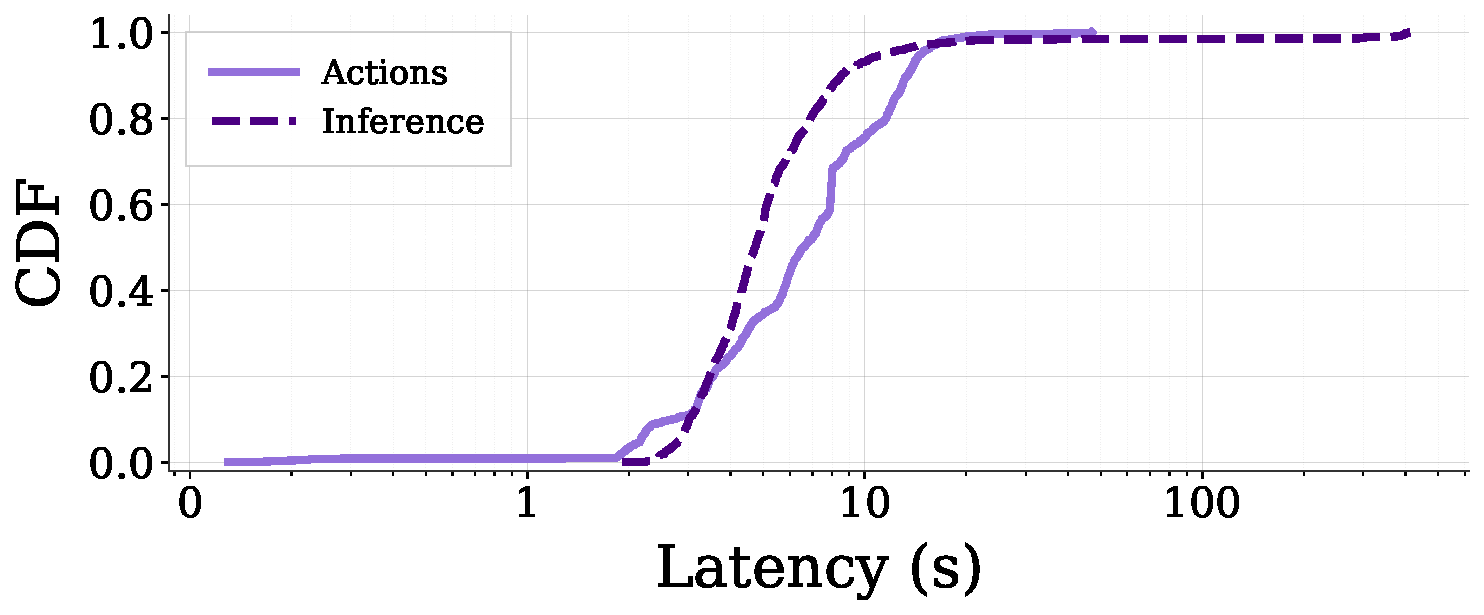
\includegraphics[width=0.8\columnwidth]{figures/latency_breakdown_cdf.pdf}
    \tightcaption{Per-step breakdown of latencies. Actions involve typing, clicking, googling, and scrolling while inference involves running the frontier model on the web input}
    \label{fig:latency-breakdown}
\end{figure}


\subsection{Overview of web agents}
\label{sec:bg}

Canonical web agents such as WebVoyager~\cite{webvoyager}, AgentOccam~\cite{agentoccam}, BrowserUse~\cite{browseruse}, and SeeAct~\cite{seeact} operate by coupling a frontier LLM with a headless browser through a ReAct execution loop~\cite{react} (Figure~\ref{fig:react-workflow}). At each step, the agent loads the current page in the browser, observes its rendered representation as either a serialized DOM tree or a screenshot, reasons about the next action to take, and executes that action against the page through standard browser primitives such as clicks, typed input, scrolling, and navigation. Every step requires a full LLM call that processes the current page representation alongside the running interaction history. The loop repeats until the agent decides the task is complete, deemed unachievable, or until a step budget is exhausted.

Web agents are designed for tasks that require navigating human-facing sites to retrieve targeted information. Example tasks include looking up product prices and availability across e-commerce catalogs, retrieving paper abstracts and citation counts from academic repositories, comparing course offerings across educational platforms, summarizing freshly-published news articles, and gathering reservation details from booking sites. They differ from tool-using agents that call structured APIs or MCP servers designed for programmatic access (e.g., coding agents acting on local files and developer tools~\cite{swt-bench, execution-agent}), and from stateless retrieval pipelines that synthesize answers from search-engine results without visiting the underlying pages~\cite{caesar}. The defining feature of a web agent is that it operates against the \emph{live web}, and must reason about page content and interaction patterns that vary across sites and across queries.


\subsection{Opportunities for specialization}
\label{sec:opp}

We start by profiling overheads across 151 representative tasks from the WebVoyager benchmark using three web agents -- BrowserUse, AgentOccam, WebVoyager -- and the experimental methodology outlined in \S\ref{sev:eval}.  Overall, we find that per-task latencies span 30-120 seconds, translating to per-task API costs of \$0.20-0.50 for model inference. Digging deeper, this overhead decomposes into two factors that each contribute substantially: the number of steps a trajectory takes, and the overhead of each step. As Figure~\ref{fig:steps} shows, the median task takes 4 steps with 80\% of tasks requiring at least 7 steps. Figure~\ref{fig:latency-breakdown} breaks down each step into browser actions and LLM inference delays, showing that both contribute meaningfully (median delays of 4.7 secs for LLM inference and 6.6 secs for browser action time, respectively). Since action decisions are conditioned on current page content and the trajectory thus far, per-step inference costs grow as history builds.



We argue that these overheads are not intrinsic to the underlying web agent tasks. Instead, they stem from applying heavy, general-purpose components -- frontier-model inference, full browser rendering, and the iterative ReAct loop, each designed for problems much broader than typical web agent tasks -- \emph{uniformly} across all steps regardless of need. We next describe three intrinsic properties of the web that make this uniformity unnecessary, and that together open the door to substantial specialization for acceleration.


\begin{figure}[t]
    \centering
    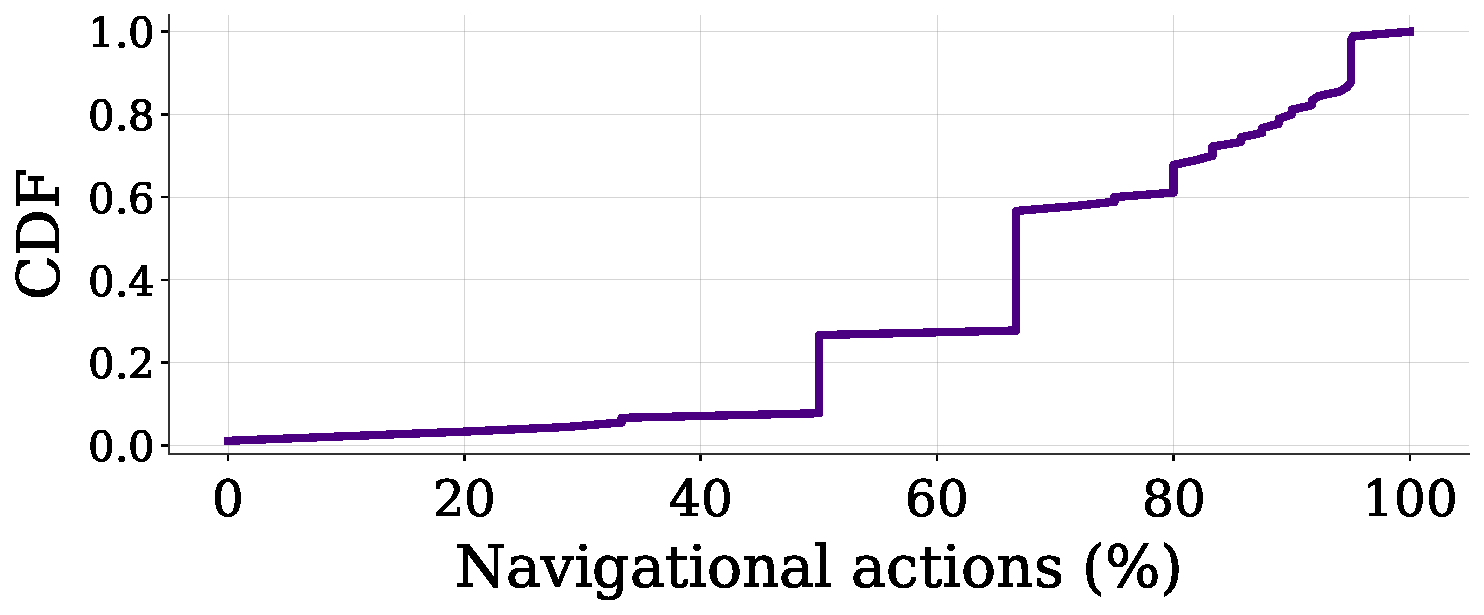
\includegraphics[width=0.8\columnwidth]{figures/navigational_actions_cdf.pdf}
    \tightcaption{Distribution of the percentage of steps per task that are navigational, i.e., moving the agent between pages rather than directly satisfying a task requirement by extracting an answer, comparing values, modifying page state.}
    \label{fig:navigational-actions}
\end{figure}

\begin{figure}[t]
    \centering
    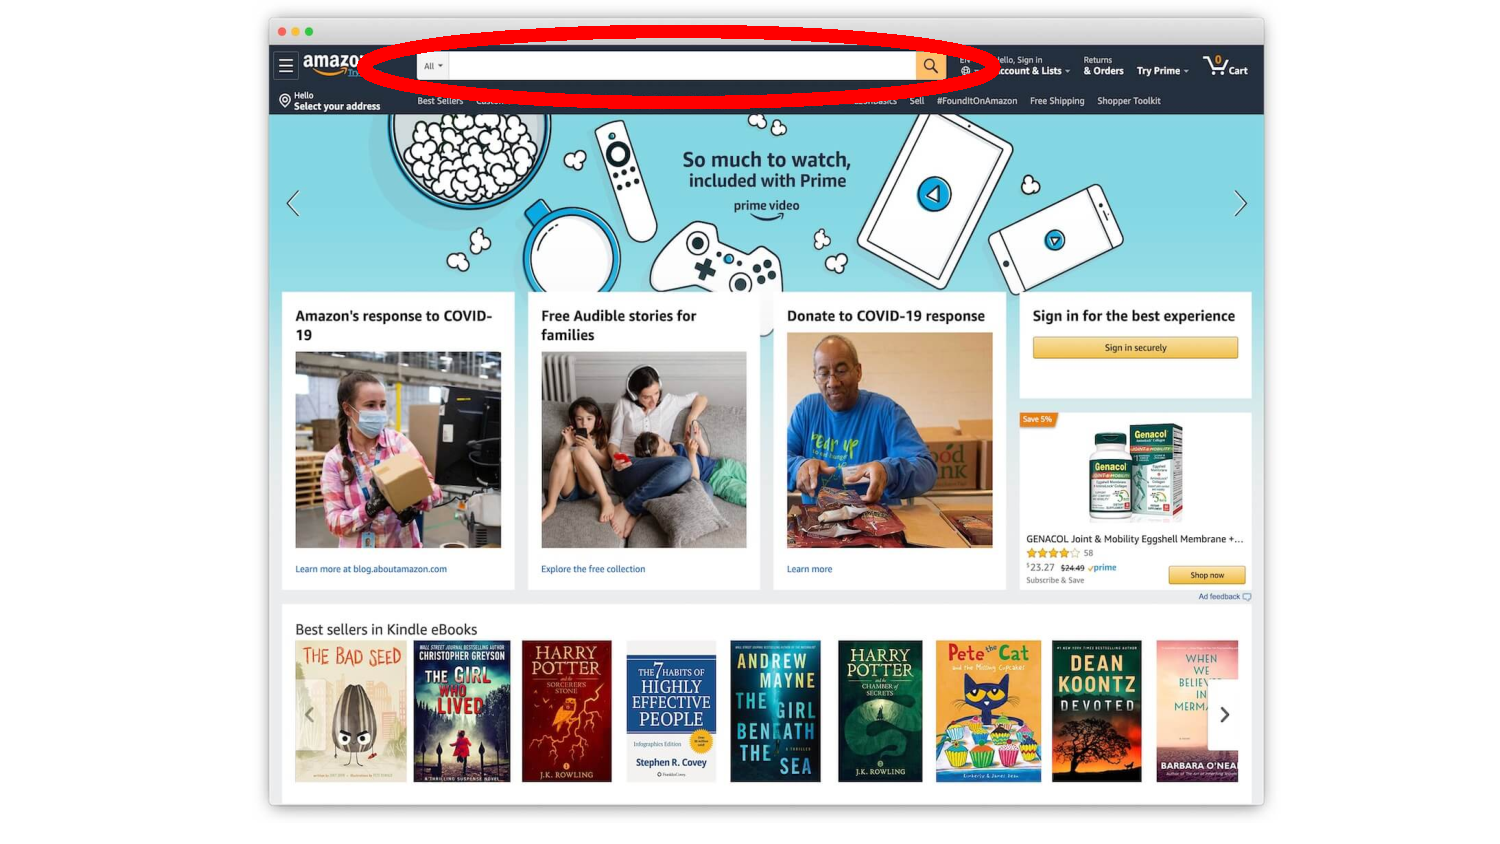
\includegraphics[width=0.8\columnwidth]{figures/excessive-data-2.pdf}
    \tightcaption{Web state input at one step of a task. Red circle marks the search bar, the only
element load-bearing for the next action (typing the query). The
rest of the input (product recommendations,
images, sidebar links, etc.) is not needed.}
    \label{fig:excessive-data}
\end{figure}


\para{Most steps are navigational.}
Most web agent tasks involve read-only information retrieval (a product price, a paper's citation count, a course's prerequisites), with the answer typically concentrated on one or a few destination pages. Reaching those pages involves searching, filtering, paginating, clicking through results, and so on. However, these steps are primarily navigational -- steps used to move between pages rather than to directly satisfy a task requirement -- rather than load-bearing reasoning. Figure~\ref{fig:navigational-actions} illustrates this, showing that 66.7\% of steps are purely navigational for the median task in our benchmarks. Further, on a given site, this navigation often follows query-invariant patterns: every Amazon shopping task involves search-then-product-page navigation, every arXiv lookup resolves an identifier to an abstract page, every GitHub task locates a repository by owner and name. An agent that knows the pattern can thus reach the destination in a single direct fetch rather than rediscovering it via a multi-step ReAct loop, with only the query-specific identifiers substituted in.

%Most web agent tasks involve read-only information retrieval (a product price, a paper's citation count, a course's prerequisites), with the answer typically concentrated on a single destination page. Reaching that page involves searching, filtering, paginating, clicking through results, and so on. However, these steps serve primarily as navigational scaffolding for interaction intuitiveness, rather than load-bearing reasoning. Further, on a given site, task-level navigation often follows query-invariant patterns: every Amazon shopping task involves search-then-product-page navigation, every arXiv lookup resolves an identifier to an abstract page, every GitHub task locates a repository by owner and name. Figure~\ref{fig:navigational-actions} illustrates this, showing tha\fillin{X\%} of steps for the median task in our benchmarks involves actions whose sole purposes is to traverse the site without extracting information or modifying page state. An agent that knows the pattern can therefore reach the destination in a single direct fetch rather than rediscovering it through a multi-step ReAct loop, with only the query-specific identifiers substituted in. 


% \begin{figure}[t]
%     \centering
%     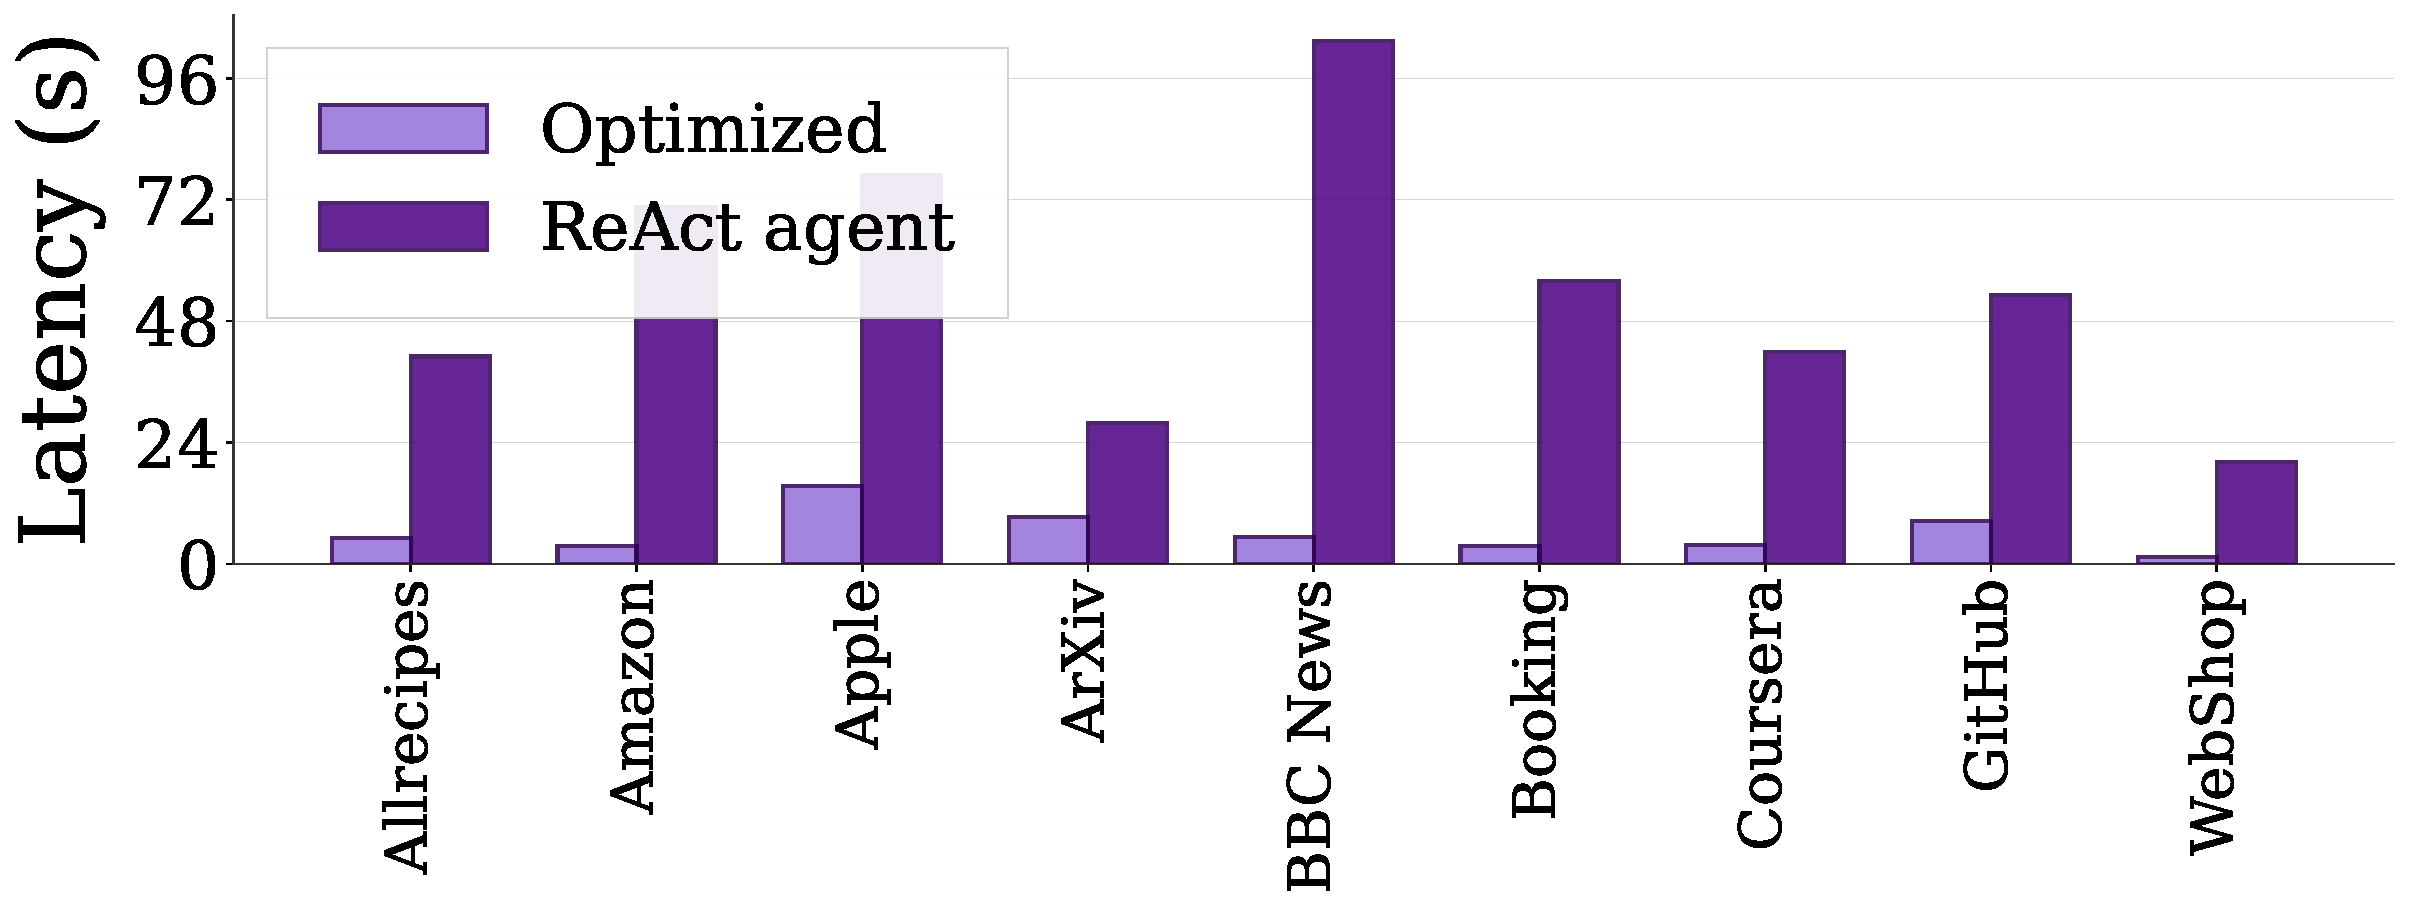
\includegraphics[width=0.99\columnwidth]{figures/hand_optimized_motivation.pdf}
%     \tightcaption{Latency of handcrafted optimized programs versus an
% off-the-shelf ReAct agent on nine representative tasks across
% diverse sites. Handcrafted programs run roughly an order of
% magnitude faster by skipping steps and using only the resources
% each task needs.}
%     \label{fig:hand-optimized}
% \end{figure}


\begin{figure}[t]
    \centering
    \begin{minipage}{0.48\columnwidth}
        \centering
        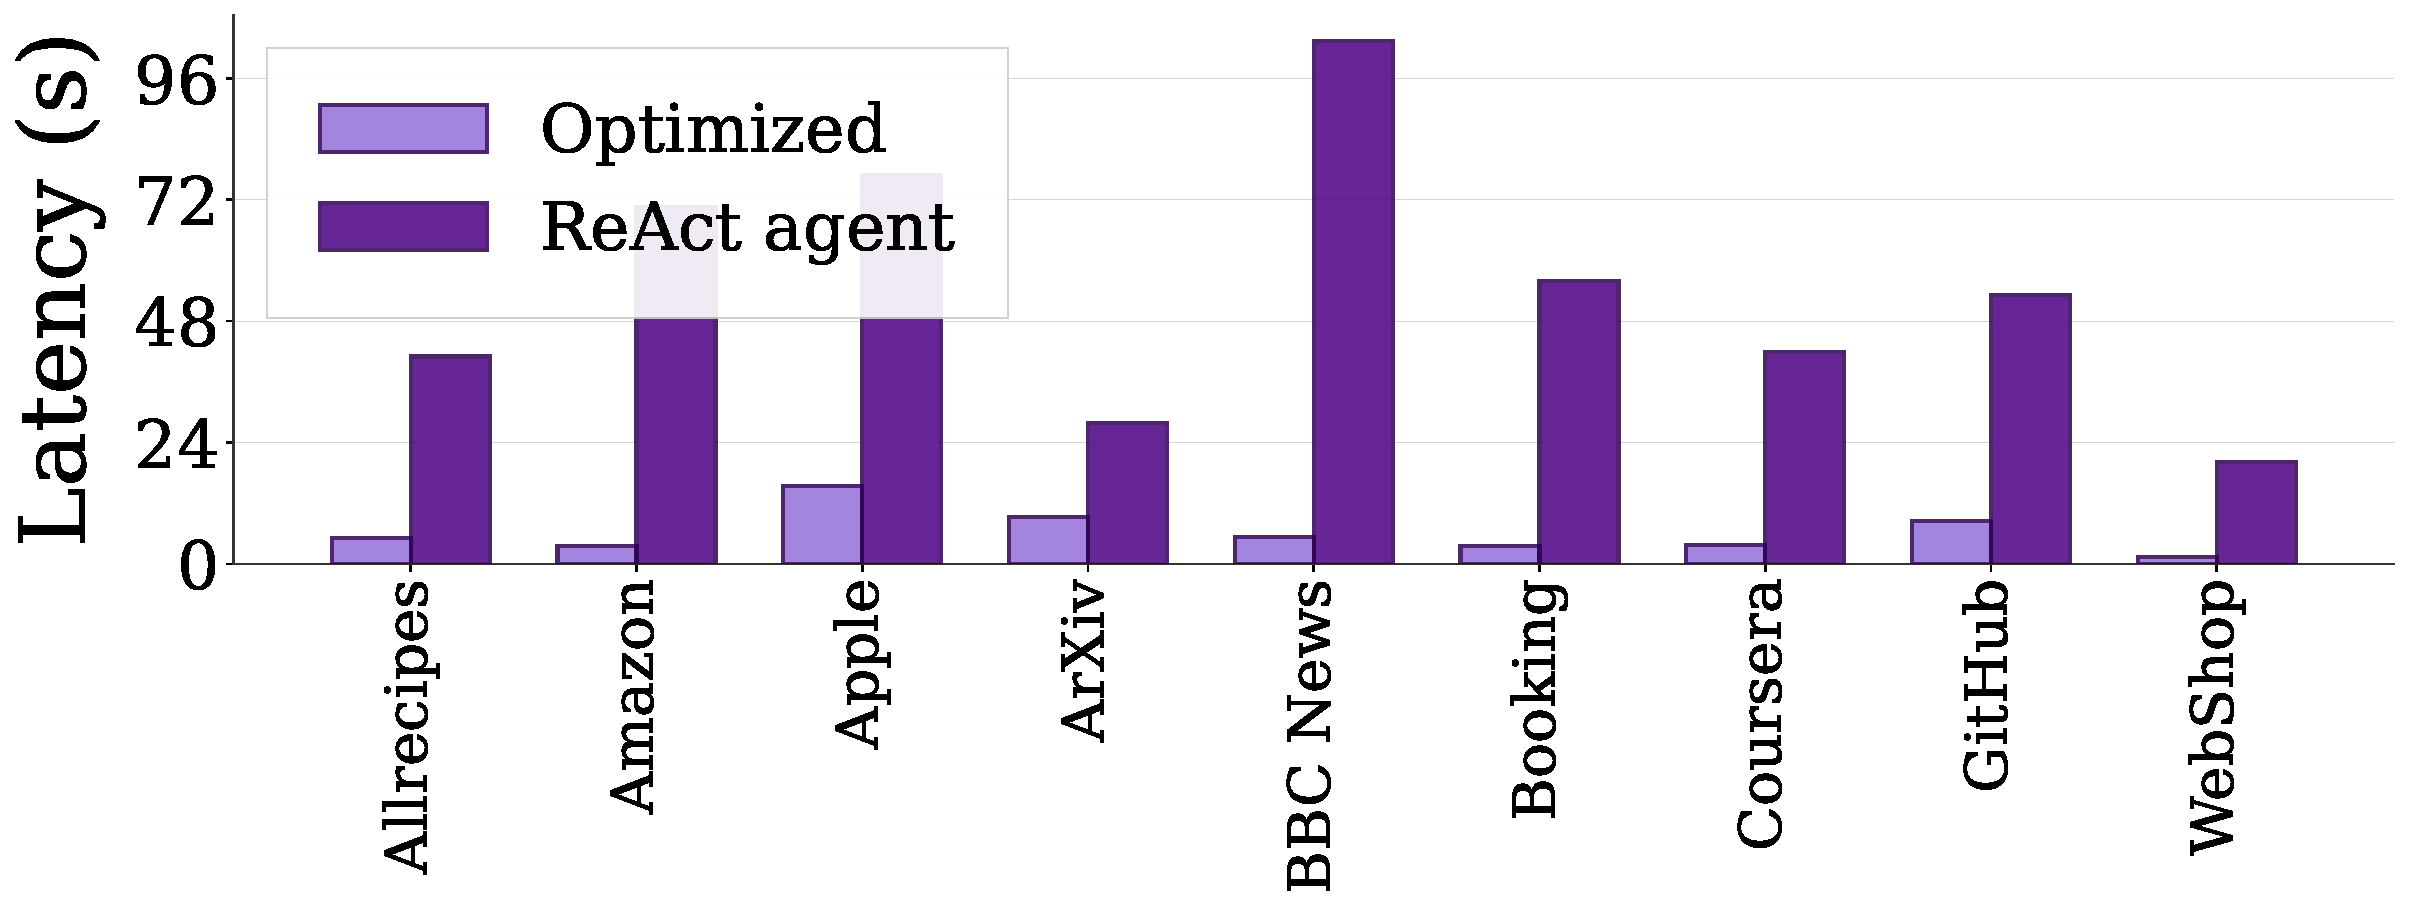
\includegraphics[width=\linewidth]{figures/hand_optimized_motivation.pdf}
        \tightcaption{Latencies of handcrafted optimized programs.}
        \label{fig:hand-optimized-latency}
    \end{minipage}
    \hfill
    \begin{minipage}{0.48\columnwidth}
        \centering
        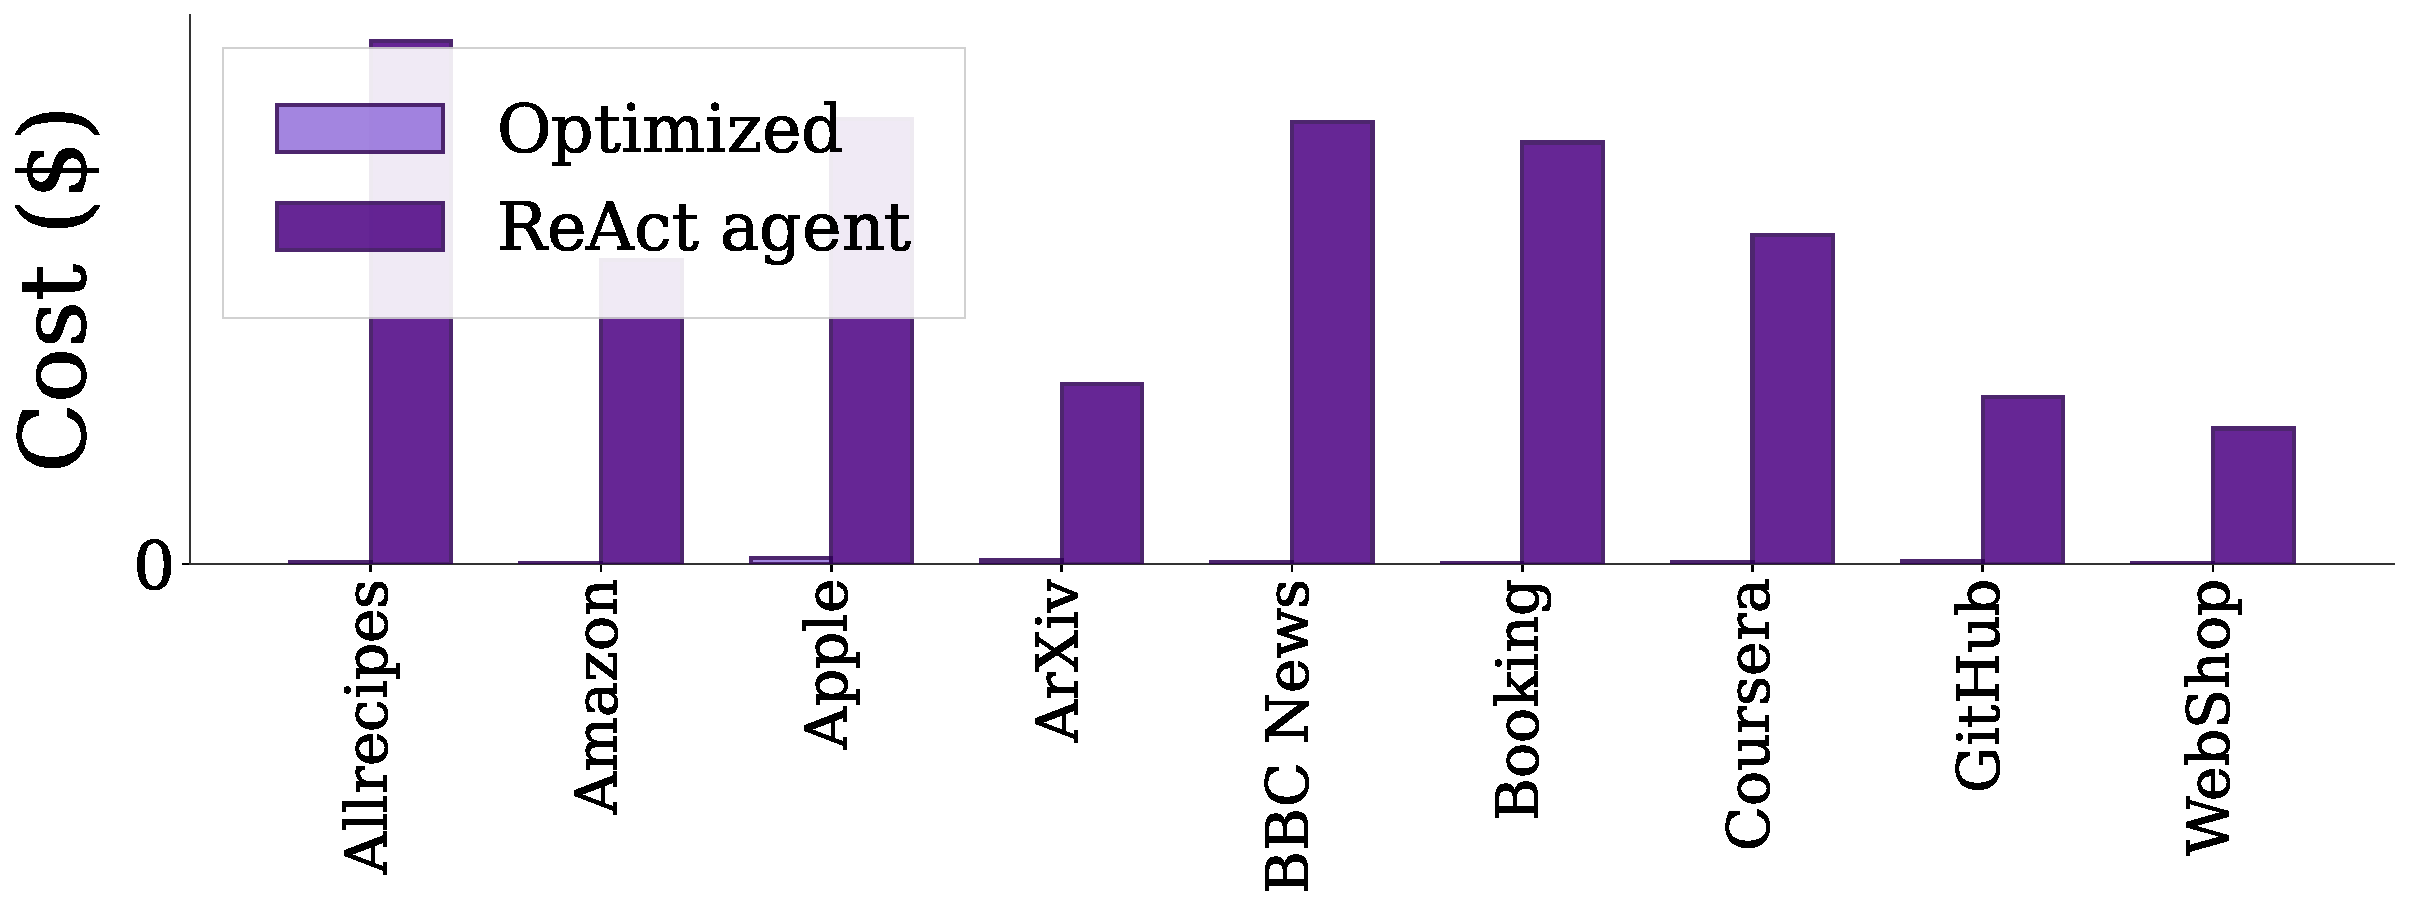
\includegraphics[width=\linewidth]{figures/hand_optimized_costs_motivation.pdf}
        \tightcaption{Costs of handcrafted optimized programs.}
        \label{fig:hand-optimized-cost}
    \end{minipage}
\end{figure}




\begin{figure}[t]
    \centering
    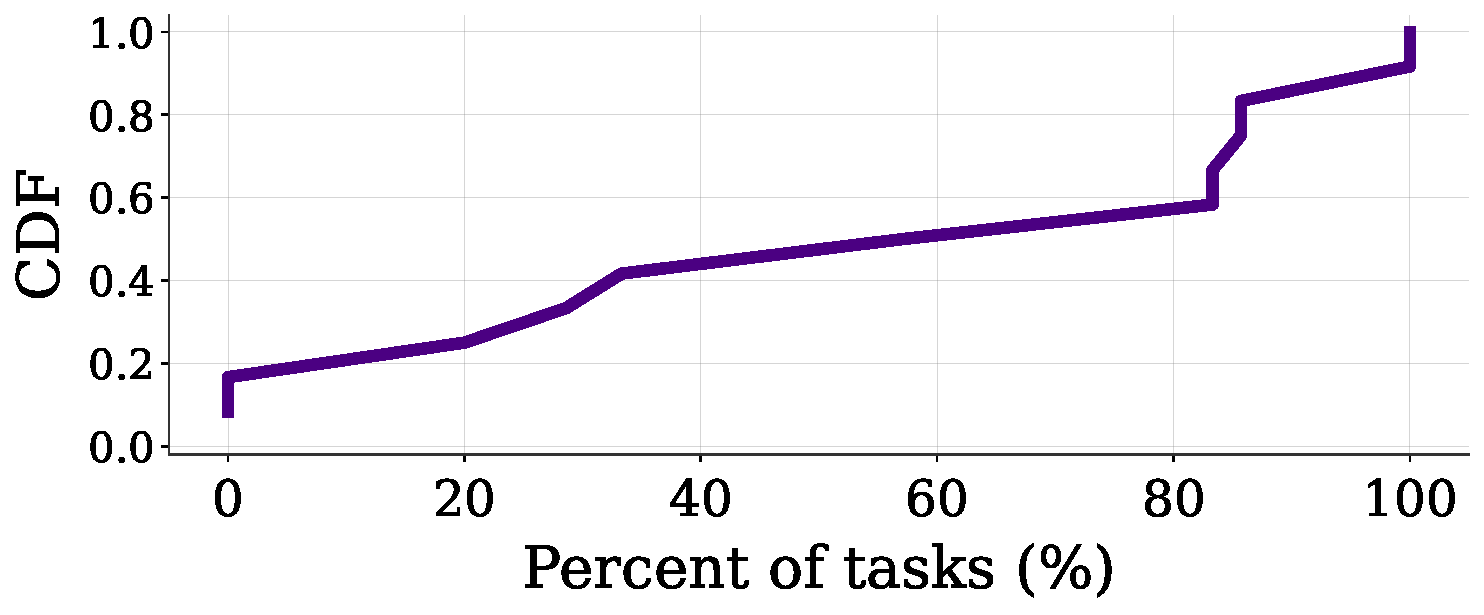
\includegraphics[width=0.8\columnwidth]{figures/http_coverage_cdf.pdf}
    \tightcaption{Fraction of tasks per site solvable via HTTP-only execution. Many sites support a large percentage of tasks through direct retrieval without browser interaction.}
    \label{fig:http-coverage}
\end{figure}

\para{Many pages do not need a browser.}
For many sites, the content embedding a task's answer is rendered on the server and arrives complete in the HTTP response body (e.g., Amazon product pages, arXiv abstracts, GitHub repository views). In these cases, a plain HTTP fetch returns what the browser would have displayed, without the high overheads of scripting and rendering. Figure~\ref{fig:http-coverage} confirms that this is common: for 55.8\% of tasks in our benchmark, the content necessary to resolve the query is fully accessible via HTTP fetch alone, without invoking the browser. Browser execution remains necessary only when client-side JavaScript produces load-bearing content (e.g., interactive maps, dynamically-revealed product variants), and even then, these overheads are warranted only for the specific steps that depend on the dynamically-generated content. Skipping even a subset of browser executions can eliminate substantial overhead.

\begin{figure}[t]
    \centering
    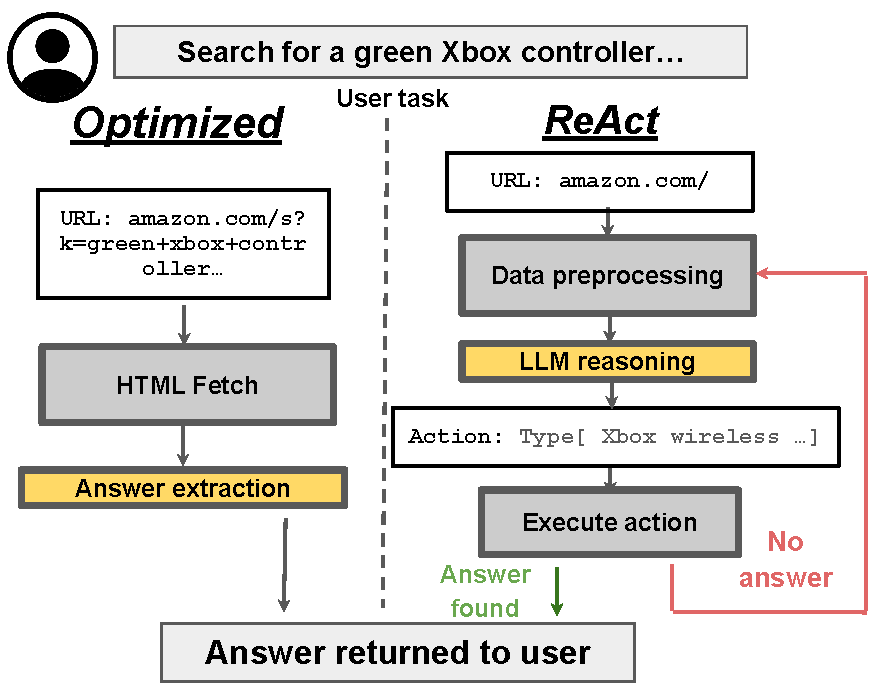
\includegraphics[width=0.8\columnwidth]{figures/optimized-web-program.pdf}
    \tightcaption{Comparison of a hand-optimized program (left) and the
corresponding off-the-shelf ReAct trajectory (right) for an
Amazon retrieval task. }
\vspace{4pt}
    \label{fig:optimized-web-program}
\end{figure}

%\para{Many pages do not need a browser.}
%For many sites, the content embedding a task's answer is rendered on the server and arrives complete in the HTTP response body (e.g., Amazon product pages, arXiv abstracts, GitHub repository views). In these cases, a plain HTTP fetch returns what the browser would have displayed, without the high overheads of scripting and rendering. Browser execution remains necessary only when client-side JavaScript produces load-bearing content (e.g., interactive maps, dynamically-revealed product variants), and even then, these overheads are warranted only for the specific steps that depend on the dynamically-generated content. Skipping even a subset of browser executions can eliminate substantial overhead in the agent's stack.


%Browsers are engineered to render arbitrary client-side behavior, much of which rarely contributes to the textual content an extraction model needs, e.g., GUI layout, click handling, hover effects, animation, JavaScript execution. Some client-side execution does produce load-bearing content (e.g., interactive maps, dynamically-revealed product variants), but for many read-only sites the answer-bearing content is server-rendered and arrives complete in the HTTP response body. A plain HTTP fetch therefore returns what the browser would have displayed on those sites. Even on sites where some pages require client-side rendering, direct-URL fetches still skip much of the trajectory, with browser execution invoked only for the steps that genuinely require it. The browser is the heaviest component in the agent's stack — both in per-step latency and in operational overhead — and many steps need none of what it provides.


%Browsers are engineered to render arbitrary client-side behavior that primarily exists to serve human interaction, e.g., GUI layout, click handling, hover effects, animation, JavaScript execution. For most read-only sites, the answer-bearing content is server-rendered and arrives complete in the HTTP response body, so a plain HTTP fetch returns what the browser would have displayed. Browser execution remains necessary for the minority of pages whose load-bearing content is produced by client-side JavaScript (e.g., interactive maps, dynamically-revealed product variants), but even on these sites, the steps that depend on browser rendering are a small fraction of the trajectory. The browser is the heaviest component in the agent's stack — both in per-step latency and in operational overhead — and most steps need none of what it provides.

%  \begin{figure}[t]
%      \centering
%      \includegraphics[width=0.9\columnwidth]{figures/denoised_motivation_bar.pdf} 
%           \tightcaption{Effect of page noise on extraction accuracy. Qwen2.5-14B matches GPT-4o on small, denoised page content embedding only the necessary information, but degrades sharply on full pages while GPT-4o remains comparatively robust.}
% %     % \tightcaption{\fillin{Accuracy with small and frontier models as additional page content not relevant to the step goal is considered during inference.}}
%      \label{fig:accuracy-vs-noise}
%  \end{figure}

 \begin{table}[t]
    \centering
    \small
    \begin{tabular}{lcc}
        \toprule
        \textbf{Model} & \textbf{Denoised environment} & \textbf{Full environment} \\
        \midrule
        Qwen2.5-14B & 42.7\%  & 26.1\%  \\
        GPT-4o &  45.7\% & 45.0\% \\
        \bottomrule
    \end{tabular}
    \vspace{8pt}
    \tightcaption{Effect of page noise on extraction accuracy. Qwen2.5-14B matches GPT-4o on small, denoised page content embedding only the necessary information, but degrades sharply on full pages while GPT-4o remains comparatively robust.}
        \label{t:accuracy-vs-noise}
\end{table}

\para{Most steps do not need a frontier model.}
A typical web page presents hundreds of potential actions in the form of interactive elements alongside ads, recommendation widgets, navigation chrome, and related-content sidebars (Figure~\ref{fig:nav-elements-challenge1}). However, the content directly relevant to a given step (e.g., a price, an abstract, a commit count) often occupies only a small fraction of the page's DOM content; Figure~\ref{fig:excessive-data} shows an illustrative example. Powerful frontier models are necessary to reason over this combination of useful content and noise, but the underlying extraction -- i.e., locating and returning the page content relevant to the step -- is not inherently hard. The relevant region is not only small but predictably located: a product's price routinely appears in the same place across product pages, an ArXiv abstract appears in the same place across paper pages, etc. Once that region is isolated, extraction reduces to a structured task within a smaller model's competence. 
Table~\ref{t:accuracy-vs-noise} confirms this empirically: when presented only with the region of a page embedding the answer (i.e., `denoised'), non-frontier models nearly match frontier-model accuracy; on full pages, however, non-frontier accuracy plummets while frontier models remain capable. 

%Powerful reasoning models have the ability to reason over the abundance of content and hundreds of action choices in a typical page (Figure~\ref{fig:accessibility-tree}) to robustly decide what to do next. However, despite the array of information that pages embed (e.g., ads, recomendation widgets, sidebars), the content directly related to the step at hand (e.g., a price, an abstract, a commit count) typically occupies a very small fraction of the page's DOM. (Figure~\ref{fig:excessive-data} provides an example). This observation has direct implications on inference costs: pages are organized so that any given query's answer often lives in a small, predictable region of the page, and once that region is isolated, the extraction itself is a structured task within a smaller model's competence. Figure~\ref{fig:accuracy-vs-noise} confirms this empirically, showing that small models rival accuracies of their frontier counterparts when presented only the necessary page content for a step, but unlike frontier models, their accuracy quickly degrades as the surrounding (noisy) page content they are presented with grows. 

%are necessary when an agent must reason over a noisy, unstructured page to decide what to do next: a typical page (Figure~\ref{fig:accessibility-tree}) presents hundreds of clickable elements alongside ads, recommendation widgets, navigation chrome, and related-content sidebars, with the step-related content (a price, an abstract, a commit count) occupying a small fraction of the DOM. The difficulty is one of noise tolerance, not of the underlying extraction: pages are organized so that any given query's answer lives in a small, predictable region of the page, and once that region is isolated, the extraction itself is a structured task within a smaller model's competence. Figure~\ref{fig:accuracy-vs-noise} confirms this empirically. When given only the answer-bearing region of a page, non-frontier models match frontier-model accuracy; as surrounding noise is added, non-frontier accuracy degrades while frontier accuracy remains roughly flat. The full-page noise is what forces frontier models in the first place. An agent that filters page content against an expected answer structure can therefore replace frontier inference with non-frontier inference on the resulting focused subset.

\para{Opportunity.}
To quantify the savings these three properties enable, we hand-engineer specialized programs for nine representative tasks in the WebVoyager benchmark. Each program implements the same recipe illustrated in Figure~\ref{fig:optimized-web-program}: a per-site URL template constructs the target page URL, an HTTP request fetches the page, the HTML is filtered to the answer-bearing region encoded by the site's expected answer structure, and a non-frontier model (i.e., Qwen2.5-14B-Instruct rather than GPT-4o/GPT-5) extracts the answer. As Figures~\ref{fig:hand-optimized-latency} and \ref{fig:hand-optimized-cost} shows, these fast-path programs run 66.7-94.9\% faster 17.7-100.7$\times$ lower costs) than the off-the-shelf ReAct agent, while preserving accuracy.

\begin{figure}[t]
    \centering
    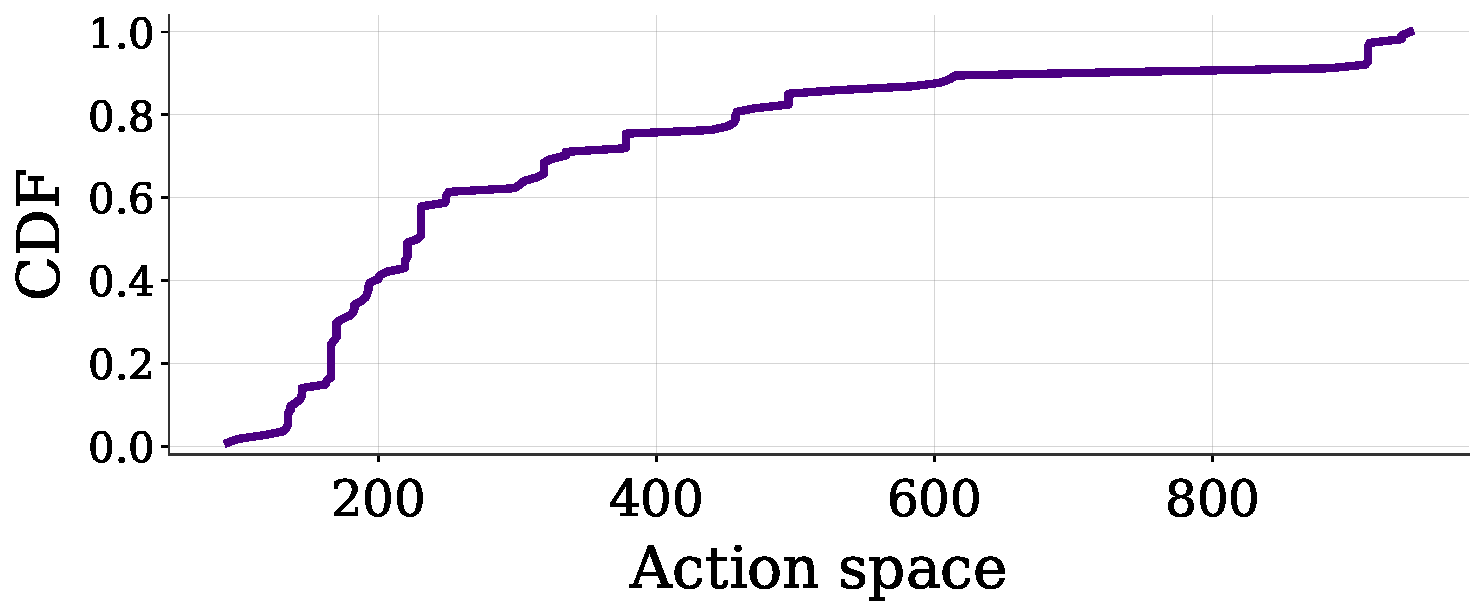
\includegraphics[width=0.8\columnwidth]{figures/action_space_count_cdf_challenge_1.pdf}
    \tightcaption{CDF of navigational elements (links, buttons, form
inputs) per page across ReAct trajectories. The median page
presents 212+ navigational elements, each leading to a different
page. }
    \label{fig:nav-elements-challenge1}
\end{figure}


\begin{figure}[t]
    \centering
    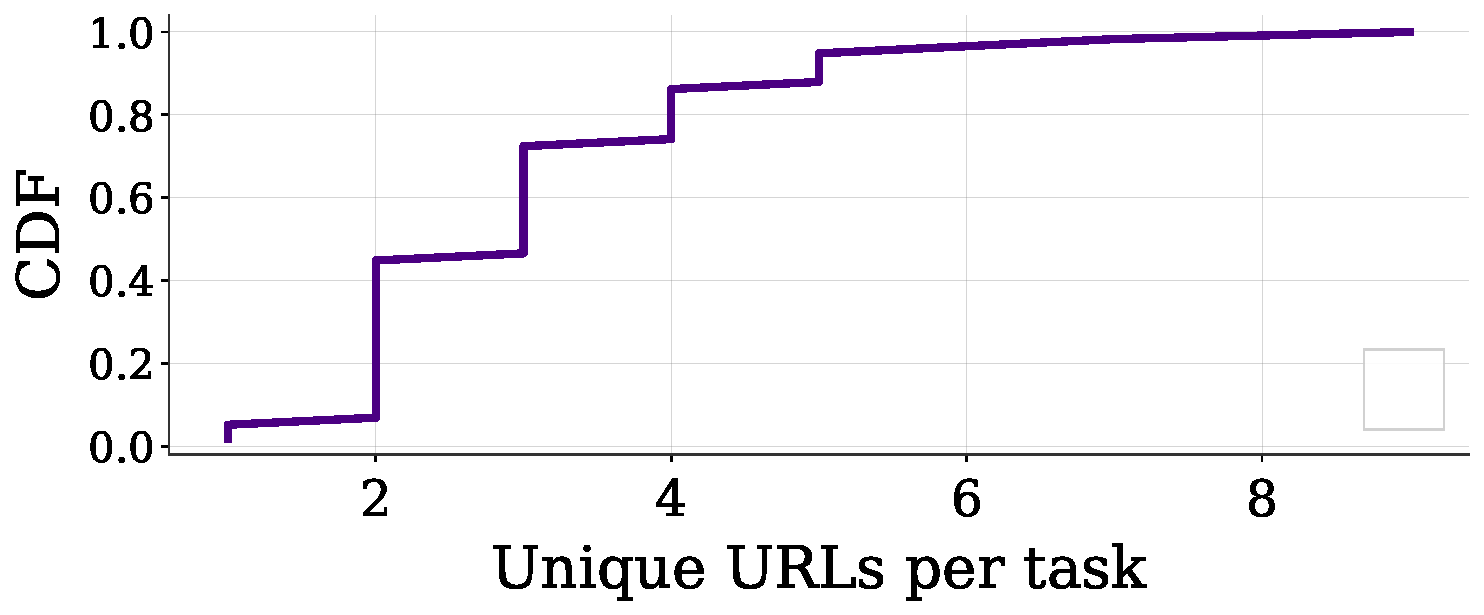
\includegraphics[width=0.8\columnwidth]{figures/unique_per_task_url_cdf_challenge1.pdf}
    \tightcaption{Number of unique URLs visited by each task. Tasks tend to take very different trajectories. Note that multiple steps often occur within each URL (e.g., scrolling) }
    \label{fig:unique-per-task-url-cdf-challenge1}
\end{figure}


\begin{figure}[t]
    \centering
    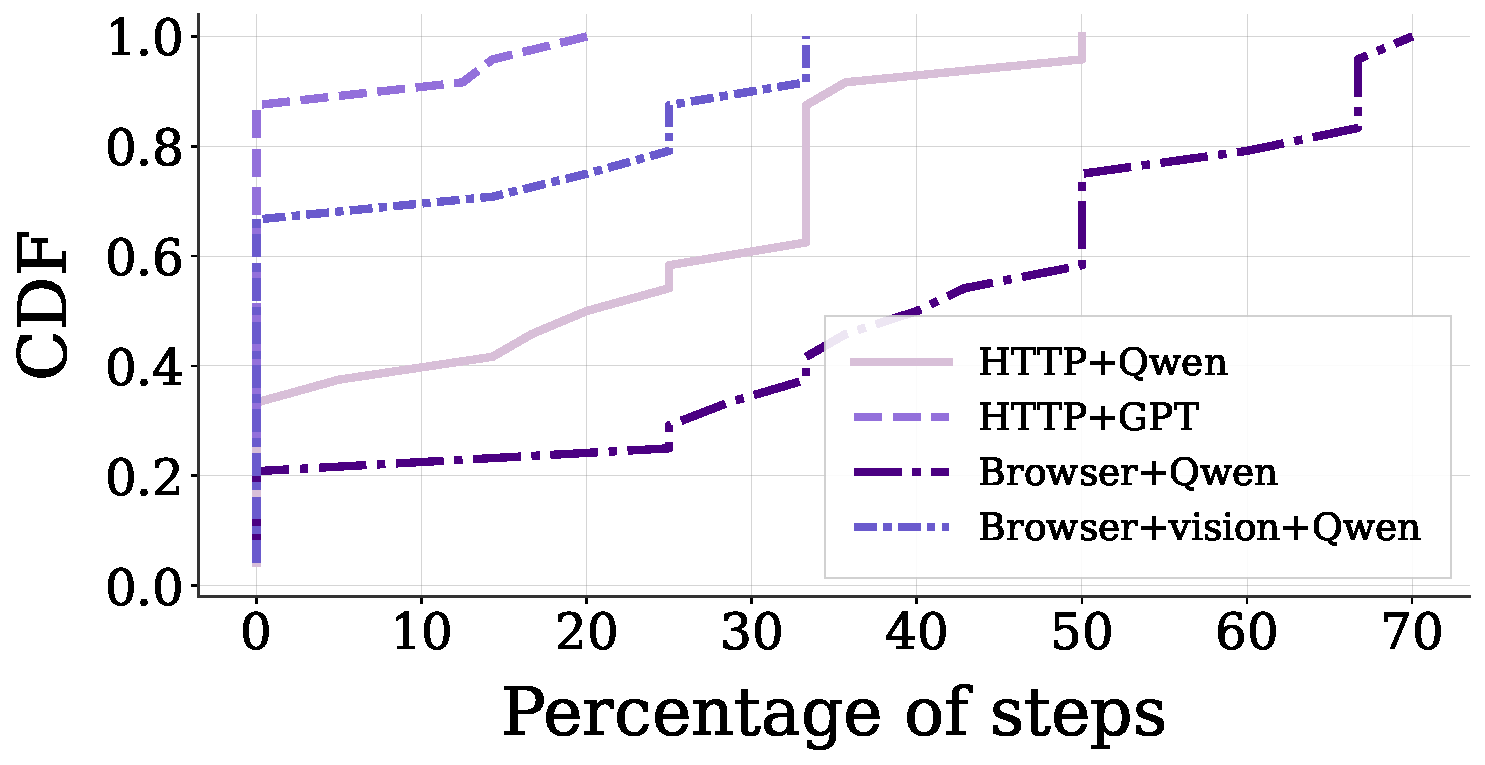
\includegraphics[width=0.8\columnwidth]{figures/minimum_tier_required_challenge_2.pdf}
    \tightcaption{CDF over tasks of the percentage of steps requiring each compute tier as the weakest tier sufficient to match the full ReAct agent. Tiers combine page-fetch (HTTP, browser, or browser w/ screenshot) with a model (Qwen2.5-14B or GPT-4o).}
    \label{fig:minimum-tier-required-challenge2}
\end{figure}

\subsection{Challenges}
\label{sec:chal}

Automatically realizing the promise of specialization above requires overcoming two key challenges, which we describe in turn. The cost of getting either wrong is severe: naively substituting cheap components (a non-frontier model and HTTP fetch) into the off-the-shelf ReAct loop, without the URL templates and answer schemas that hand-engineered programs encode, drops average task success by 60\% since errors compound across the trajectory and a single wrong step can invalidate everything downstream.

%The cost of getting either wrong is severe: naively applying the recipe of fast optimizations in Figure~\ref{fig:optimized-web-program} to the off-the-shelf ReAct loop drops task success to 0\%, since errors compound across the trajectory and a single wrong step can invalidate everything downstream.


\para{C1: Determining \emph{what} can be specialized.}
Before execution begins, the agent must determine which parts of an incoming task support specialization, i.e., which trajectories can be replaced by direct URL fetches, which pages can be served without a browser, and which extraction steps can use a non-frontier model. This determination is hard for two reinforcing reasons. First, the signal available at query time is thin. Task text describes user intent (``find the cheapest blue headphones'') rather than the trajectory pattern that resolves it, and even on a single site, different tasks visit different pages through different navigation sequences. Second, recognition itself has a cost ceiling: if identifying reuse opportunities requires running a frontier model over the full site or comparing against a large trajectory database, the cost of recognition negates the savings that the specialization would yield. The challenge is thus how to encode reusable site structure ahead of time and match incoming tasks against it efficiently at runtime.

%\emph{robustly} surface reusable site structure ahead of time and recognize when an incoming task matches it cheaply enough that the savings remain meaningful.


\para{C2: Determining \emph{how} to specialize across steps.}
Even when specialization applies, the minimum-cost \emph{tier} -- a combination of retrieval, rendering, and extraction model -- sufficient to match the default agent varies per step within a single trajectory. Figure~\ref{fig:minimum-tier-required-challenge2} highlights this by showing the distribution of minimum-tier support needed across task steps. As shown, some steps are resolved by the cheapest tier (HTTP fetch with a non-frontier model), others require browser rendering to access client-side content, others require a frontier model for extraction the small model cannot perform, and some require both. Importantly, the variation is \emph{per step}, not just per task; even tasks amenable to specialization mix step types within their trajectories. Choosing the wrong tier at any step drops accuracy substantially. For instance, a small model handed a raw DOM with a complex extraction task might return the wrong field, while an HTTP fetch of a JavaScript-dependent page will return a content stub without the necessary information. The challenge is to determine the minimum sufficient tier per step without paying the cost of running the default agent to find out.




\begin{figure*}[t]
    \centering
    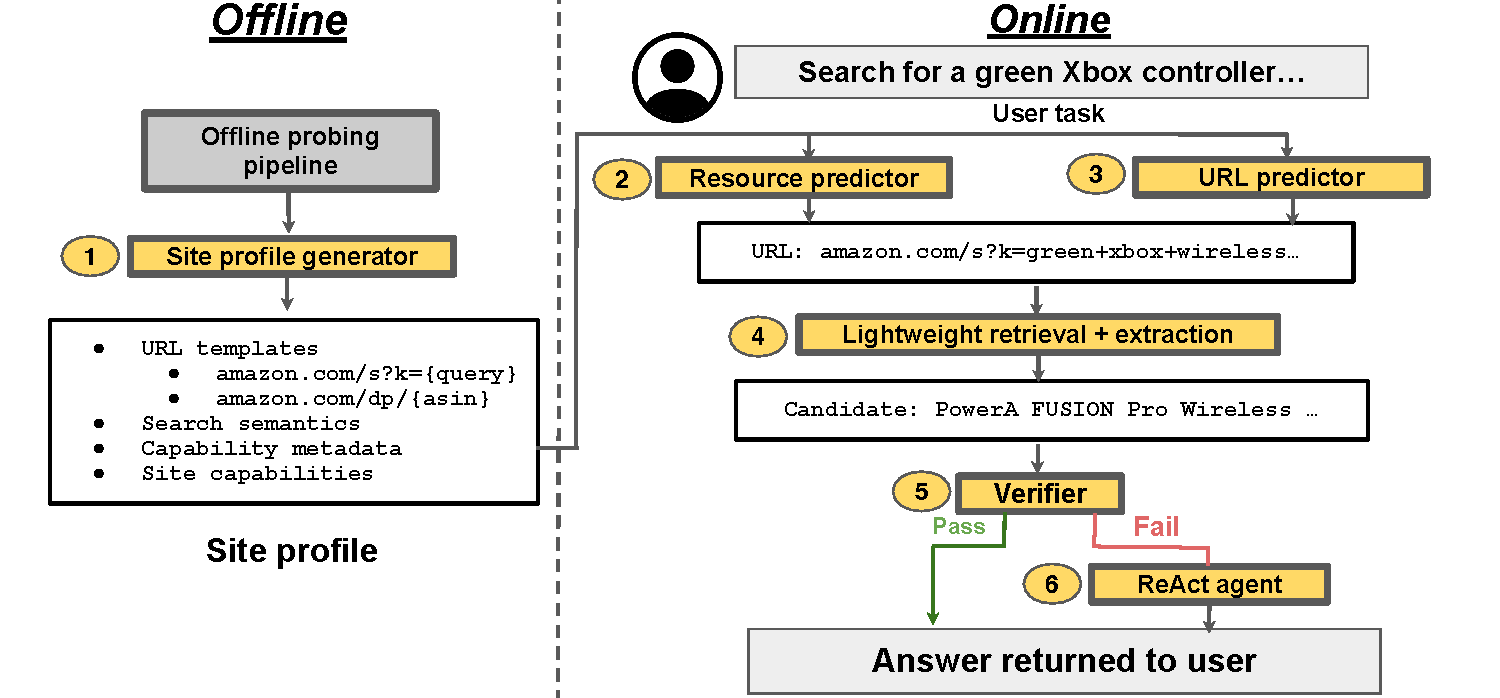
\includegraphics[width=0.8\textwidth]{figures/web-agent-workflow.pdf}
    \tightcaption{\sys end-to-end. Offline (left): a profiling pipeline
    encodes per-site URL templates, search behavior, and extraction
    schemas into a reusable site profile. Online (right): tasks attempt
    direct addressing through template-driven URL synthesis, plain HTTP
    fetch, and lightweight extraction. Output is verified before
    commitment; on rejection, the system cascades to a heavier
    execution tier resuming at the URL the fast path reached.}
    \label{fig:design}
\end{figure*}

% =============================================================================
\section{Design of \sys{}}

\subsection{Overview}
To address these challenges, we introduce \sys{}, a framework that accelerates web agents through speculative lightweight execution while preserving robustness through verification and selective escalation only when needed. Figure~\ref{fig:design} illustrates \sys{}'s end-to-end operation. The system rests on two complementary observations about purpose-built websites. First, website structure is sufficiently stable that reusable navigation patterns, search semantics, and capability characteristics can be extracted offline and amortized across future queries. Second, most read-only web tasks do not require full iterative browser interaction — they can often be resolved through direct retrieval and lightweight extraction once the correct URL and execution environment are known. \sys{} therefore combines offline structural profiling with an online speculative cascade: offline profiling provides reusable trajectory priors, while runtime verification and fallback preserve correctness when speculation fails. These two mechanisms jointly address C1 and C2; offline patterns alone are insufficient because websites contain unpredictable edge cases, while runtime adaptation alone lacks the structural priors needed to make speculative execution efficient.

\sys{} interposes between the user and an underlying ReAct agent. Before runtime, an offline profiling stage \textcircled{1} constructs per-site profiles encoding URL templates, search semantics, pagination behavior, query-construction guidance, and execution-relevant capability metadata. For each incoming task, a capability and resource predictor \textcircled{2} determines the minimum execution environment and reasoning resources likely required, while a structure predictor \textcircled{3} attempts to synthesize a high-probability retrieval URL using the site profile. The system then performs lightweight retrieval and extraction \textcircled{4}, fetching the page through the cheapest supported mechanism and running schema-guided extraction over cleaned HTML. A verifier \textcircled{5} checks whether the speculative result is consistent with the task: if verification succeeds, the answer is returned immediately; otherwise, execution escalates to the full ReAct agent \textcircled{6}, seeded with the speculative URL as a warm start to preserve navigational progress. Tasks that match no reliable template, as well as state-mutating tasks outside the read-only scope (\S\ref{sec:background}), bypass speculative execution and route directly to the default ReAct agent. We describe offline profiling pipeline in \S\ref{sec:design:offline}, and runtime cascade in \S\ref{sec:design:runtime}.

\sys's speculation primitive admits two deployment policies. In accelerate mode, a verified fast path commits immediately and the saved compute is returned to the user as reduced latency and cost. In aggregate mode, the saved budget is reinvested into additional speculative trials within the baseline's single-execution cost envelope; the verifier ranks the resulting candidates and selects the best. Both modes share the same offline profiles, runtime URL synthesis, and verifier; they differ only in what is done with the verifier's output. Accelerate mode treats verification as a commit gate; aggregate mode treats it as a ranking function. 

\subsection{Offline Profiling Pipeline}
\label{sec:design:offline}

The offline pipeline produces a per-site profile that captures
reusable trajectory structure. Site URL patterns and structural
conventions are stable across queries, e.g., Amazon products are
addressable by a stable product identifier (Amazon Standard
ID), arXiv papers by identifier,
and GitHub repositories by \texttt{owner/repo}. The profile can
thus be built once per site and reused across subsequent
tasks. This stability is what makes C1's prediction problem
tractable despite thin task-time signal: rather than inferring
reusable patterns at runtime from task text and a brief view of
the site, the system matches each task against an already-built
site profile.

\para{What a profile contains.}
A site profile encodes the reusable structural information \sys{} needs to specialize execution. %Figure \ref{fig:site-profile} in Appendix \ref{s:appendix} shows a compressed excerpt; 
The profile contains rich search semantics, pagination behavior, capability measurements, extraction schemas, verification metadata, and query-construction guidance. Each profile has four main components. First, typed URL templates capture reusable navigation patterns (direct identifier lookup, filtered search, sorted retrieval, paginated traversal); each template contains parameterized URL patterns and regex constraints that map natural-language task descriptions into site-valid parameter values. Second, search semantics encode how a site constructs queries, exposes filters, handles sorting and pagination, signals empty results, and maps structured attributes (e.g., price ranges, categories, authors, difficulty levels) into URL parameters. Third, answer schemas specify the expected structure and types of valid responses, enabling both focused extraction and lightweight runtime verification. Fourth, capability metadata records execution-relevant properties measured during probing: JavaScript dependence, HTTP accessibility, bot-detection behavior, rendering constraints, response latency, and content-density statistics.

Profiles also store compact query-construction notes and representative search queries generated offline, guiding runtime URL synthesis toward high-coverage search paths without overwhelming downstream models with large template spaces. The goal is not to memorize every possible trajectory, but to capture the small set of structurally common navigation patterns that cover most realistic tasks.

\para{How profiles are constructed.}
Profiles are generated by an automated offline probing pipeline that runs once per site. The pipeline characterizes the site's execution environment through lightweight HTTP probing, measuring response latency, visible-content density, HTTP accessibility, and bot-detection behavior; when HTTP retrieval returns sparse or incomplete content, it escalates to a headless browser to recover the fully rendered page. Using the best available HTML, it then discovers search endpoints by analyzing form structure and common search-URL conventions, identifies pagination behavior by traversing result pages, and validates candidate URL templates against real site behavior. Rather than enumerating all possible trajectories, the prober strategically searches for reusable structural patterns that maximize coverage across common task classes while keeping the template space compact for efficient runtime matching. This reflects an empirical property of purpose-built sites: although URLs and content vary enormously across queries, the underlying navigation mechanisms are highly similar — product sites repeatedly expose search, filter, sort, and pagination flows; literature sites repeatedly expose identifier lookup and query retrieval flows; repository sites repeatedly expose repository, issue, and commit navigation flows.

The pipeline further enriches each profile using a local LLM that analyzes discovered search endpoints, validated URL patterns, and representative task descriptions to synthesize query-construction guidance and representative search queries. These enrichment stages help \sys{} learn which task attributes are structurally useful for retrieval on a given site and which are likely to hurt coverage or overconstrain search. For example, shopping sites benefit from including product attributes (color, material, device type), while review-count thresholds or highly specific descriptive modifiers often reduce retrieval quality. The resulting profiles therefore encode not only URL structure but also higher-level retrieval strategies specialized to each site's intended purpose.

\para{Handling site changes.} Site profiles persist for long periods without growing stale. While dynamic content changes continuously (Amazon rotates products hourly, arXiv publishes new papers daily), structural scaffolding -- search endpoints, URL parameter conventions, pagination behavior, navigation flows, and answer-bearing page layouts -- evolves much more slowly because it is tied to the site's core purpose, and the workflows that purpose supports remain stable over time. \sys exploits this asymmetry: profiles encode the slow-changing structural layer while leaving dynamic content to be resolved online at runtime.


Structural drift is therefore uncommon but not ignored.
\sys{} continuously validates profile correctness during runtime
execution through schema verification, HTTP status monitoring,
and content-consistency checks. Missing expected fields,
repeated verification failures, unexpected page structures, or
persistent HTTP errors (e.g., 404 responses on previously valid
templates) are treated as indicators that a profile may have
become stale. When such signals exceed a threshold, \sys{}
automatically re-invokes the offline probing pipeline to
regenerate the affected portions of the profile. Because
regeneration is amortized across all future tasks on the site,
occasional reprofiling incurs negligible overhead relative to
sustained query volume.


\para{URL synthesis.}
URL synthesis is the runtime mechanism that maps a task description to a URL using the profile's templates. It has two steps: selecting the right template (search vs direct lookup, with which filters and sort orders applied) and extracting parameter values to slot in (query keywords, identifiers, filter values). On Amazon, ``find the cheapest blue headphones under \$100'' selects the price-range search template with price-ascending sort, extracts ``blue headphones'' as the query and ``\$100'' as the maximum price (converted to cents per the template's parameter description), and produces ``{\nolinkurl{amazon.com/s?k=blue+headphones\&rh=p\_36\%3A0-10000\&\\s=price-asc-rank}}''. The synthesized URL collapses several steps the default agent would otherwise execute through multi-step navigation (search, filter, and sort).

URL parameters codify much of a site's interactive surface (search keywords, filter values, sort orders, navigational pages), so a synthesizer that handles parameters correctly can reach most of the destinations the default agent would. \sys{} performs template selection and parameter extraction with a non-frontier model, supported by per-template regex patterns in the profile: the model proposes candidate values from the task text, and the regexes sanity-check them against the site's expected vocabulary before URL construction. The regexes are the bridge between natural-language tasks and structured URL parameters, reducing the model's job to pick the right template and surfacing the right value spans.

A non-frontier model suffices due to the structured nature of purpose-built sites. Although natural-language queries are arbitrary in principle, the \emph{semantically reasonable} queries for a given site are much narrower than the unrestricted space — nobody asks to read a research paper on Amazon or compare iPhone prices on arXiv. The site's purpose constrains the queries the synthesizer must handle to a set whose parameter types are encoded in the profile, so the model never needs to handle truly arbitrary intent. A general-purpose URL constructor that handles arbitrary tasks across arbitrary sites would benefit from a frontier model; a per-site synthesizer operating within its site's intended vocabulary does not.


\begin{figure}[t]
    \centering
    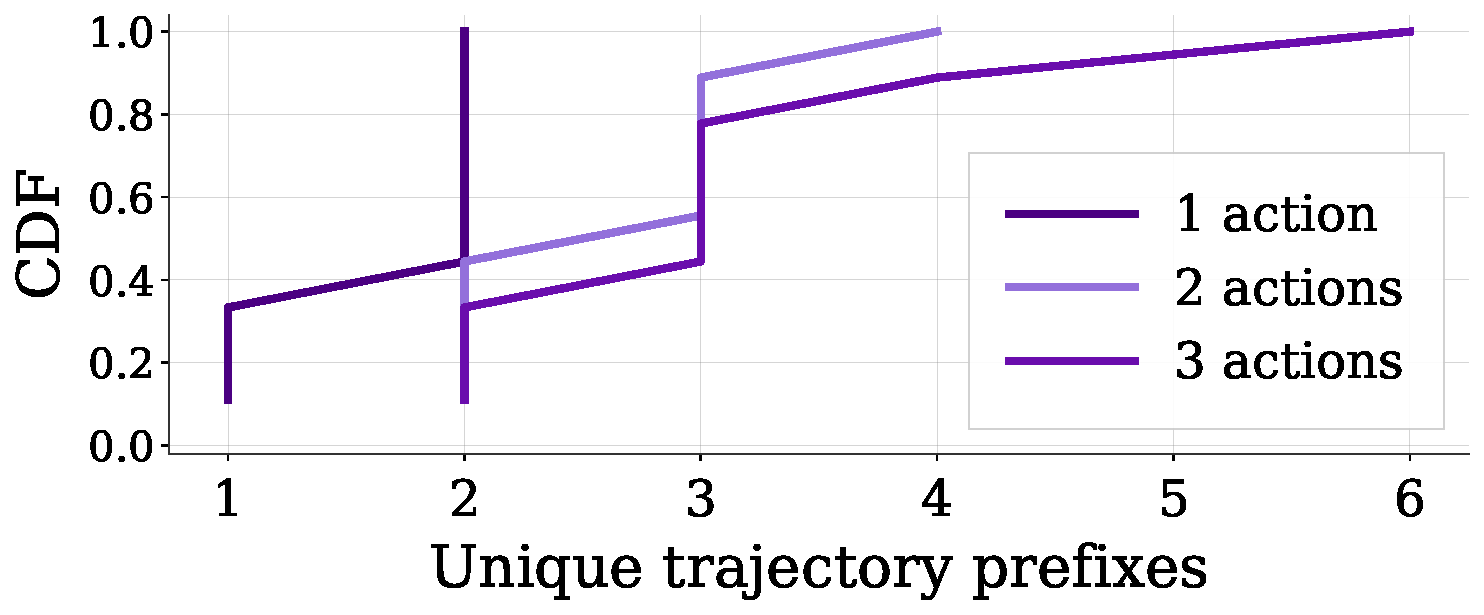
\includegraphics[width=0.99\columnwidth]{figures/trajectory_prefixes_cdf.pdf}
    % \vspace{-2em}
    \tightcaption{Distribution of the number of unique action-type prefixes across tasks on a site, for the first 1, 2, and 3 actions of each task. Prefixes consider action types (e.g., click, type), ignoring parameters like element identifiers or extracted content.}
    \label{fig:trajectory-prefixes}
\end{figure}

\subsection{Runtime Speculation}
\label{sec:design:runtime}
% The runtime cascade begins when a task arrives. \sys{} matches
% the task text against the profile's templates and slot-fills
% from the task description: ``find the abstract of arXiv paper
% 2401.12345'' matches the direct-identifier template with slot
% \texttt{2401.12345}; ``find the cheapest blue headphones on
% % Amazon'' matches the search-query template.\sn{How robust/general is this matching? strict string match? regex matching? LLM-based matching? } If no template
% matches, the task routes directly to the default ReAct agent. If
% a template matches, \sys{} determines the minimum resources the
% task requires from the profile, executes, verifies the output,
% and escalates resources on rejection.

%\begin{sloppypar}
When a task arrives, \sys matches the task against the profile's typed templates through a hybrid process: a lightweight LLM performs intent classification to select a candidate template class (e.g., direct identifier lookup, filtered search, paginated retrieval), while profile-defined regex constraints and parameter validators ground extracted slot values into site-valid parameters. The LLM thus handles semantic interpretation while typed parameter constraints enforce structural validity and prevent free-form generation. For example, ``find the abstract of arXiv paper 2401.12345'' matches the direct-identifier template with slot \texttt{2401.12345}, while ``find the cheapest blue headphones on Amazon'' matches the filtered search template with query, sort-order, and optional price slots. This combination is more robust than strict string or regex-only matching, and more reliable and cheaper than unconstrained frontier-model trajectory planning.
If no template matches with sufficient confidence, the task routes directly to the default ReAct agent. Otherwise, \sys determines the minimum resources the task requires from the profile, executes the speculative fast path, verifies the output, and escalates resources on rejection.
%\end{sloppypar}

%Runtime speculation cascade begins when a task arrives. \sys{} first matches the task text against the profile’s typed templates and extracts candidate slot values from the task description. The matching process is hybrid rather than purely symbolic: lightweight LLM-based intent classification selects candidate template classes (e.g., direct identifier lookup, filtered search, paginated retrieval), while profile-defined regex constraints and parameter validators ground the extracted slots into site-valid parameter values. For example, find the abstract of arXiv paper 2401.12345'' matches the direct-identifier template with slot \texttt{2401.12345}, while find the cheapest blue headphones on Amazon'' matches the filtered search-query template with slots corresponding to the query string, sort order, and optional price constraints. The LLM therefore performs semantic interpretation of the task, while the profile’s typed parameter constraints enforce structural validity and prevent unconstrained free-form generation. This combination makes matching substantially more robust than strict string matching or regex-only approaches while remaining more reliable and lower-cost than unconstrained frontier-model trajectory planning.

%If no template matches with sufficient confidence, the task routes directly to the default ReAct agent. Otherwise, \sys{} determines the minimum resources the task requires from the profile, executes the speculative fast path, verifies the output, and escalates resources on rejection.


Resource determination operates along three axes that govern how
a task is executed:
\begin{sloppypar}
\begin{itemize}
    \item \textbf{Page acquisition.} Either direct URL fetch
    (the page is reachable by URL synthesis from the profile
    template) or multi-step navigation (the ReAct loop). The
    profile dictates which is applicable for the task class.
    \item \textbf{Page rendering.} Either HTTP-only fetch or
    browser-driven rendering. The profile encodes which pages
    on a site require browser rendering (client-side JavaScript,
    authenticated state); pages flagged as HTTP-reachable use
    HTTP, the rest use the browser.
    \item \textbf{Reasoning model.} Either a non-frontier
    extraction model or a frontier model. The profile's answer
    schema and the cleaned page content together determine
    whether the non-frontier model can extract reliably; otherwise a frontier model is used.
\end{itemize}
\end{sloppypar}

The cheapest combination the profile justifies is tried first.
On verification failure, \sys{} escalates the axis the verifier
signals is at fault: a rejection on a missing-but-expected field
escalates the reasoning model, a rejection on an empty or blocked
page escalates rendering to the browser, and persistent failure
escalates page acquisition to full ReAct. Escalation is not a
strict hierarchy; different tasks exercise different axes. Some
need browser rendering with a non-frontier model, others need
HTTP with a frontier model, and many need only the cheapest
combination on all three. The verifier is the feedback signal
that drives axis-specific escalation rather than blind progression
through fixed tiers.

%Two empirical observations about the web domain motivate the
%verifier and warm-start design. First, trajectories on a single
%site share structural prefixes even when their task-specific
%tails differ, so a cheap path that fails has typically still
%completed real navigational progress that recovery can inherit.
%Second, verification on read-only tasks is structurally cheap:
%a site's templates, a task, and a short summary of where the
%agent landed carry enough evidence to confirm or reject without
%re-traversing the page. The first motivates the warm-start
%cascade, which inherits the URL the failed attempt reached. The
%second makes a fast-path verifier viable within the cost
%envelope the cheap path establishes.

This feedback-driven escalation rests on two empirical properties of purpose-built websites: trajectory prefixes are highly predictable, making failed speculation useful, and verification is highly constrained, making it cheap to evaluate.

%\para{Trajectories share structural prefixes.} Because sites are purpose-built around consistent interaction patterns (\S\ref{sec:opp}), trajectories on a site share a structural prefix even when their task-specific tails differ. This split matches Accio's offline/online structure: the shared prefix is what the offline profile encodes, while task-specific tails are what runtime synthesis instantiates. The cheap execution path is therefore well-suited to the structural prefix and progressively less well-suited as trajectories enter their task-specific tails. Even when the cheap path eventually fails, it has typically completed real navigational progress that can be inherited by recovery.

\para{Trajectories share structural prefixes.} On purpose-built sites, queries with different end goals typically begin with identical navigational steps (e.g., search, filter, sort) (Figure \ref{fig:trajectory-prefixes}). This split aligns with \sys{}'s offline/online design: the offline profile captures the shared prefix, while runtime synthesis executes the task-specific tail. Because the speculative fast path excels at navigating these common prefixes, even a trajectory that ultimately fails usually reaches a useful intermediate URL. A more expensive recovery policy can then inherit this progress rather than starting from scratch.


%Although different tasks produce different specific trajectories (different URLs, different parameters, different content), those trajectories share a structural prefix because sites are purpose-built around consistent interaction patterns. Two Amazon shopping tasks visit different specific product pages but both pass through the same sequence of action types: search, navigate from results, land on a product page. Two arXiv tasks fetch different specific papers, both via the same identifier-based URL construction. Two GitHub tasks visit different repositories, both resolved through the same \texttt{owner/repo} pattern. The shared structure is what the offline profile encodes; the task-specific tails (which product, which paper, which repository) are what runtime synthesis instantiates. The cheap execution path is therefore well-suited to the structural prefix and progressively less well-suited as trajectories enter their task-specific tails. Even when the cheap path eventually fails, it has typically completed real navigational progress before failing, and that progress can be inherited by recovery.

%\para{Verification is structurally cheap.}
%Two properties keep verification cheap. First, the verifier has a strong prior: the site supplies the set of structurally valid trajectory templates, and the task selects which one applies. A verifier presented with 'find my last order' and a state summary placing the agent on the orders page recognizes alignment; the same verifier with 'find the cheapest blue headphones' and the same state summary recognizes deviation. Second, web state and answers compress cleanly enough to verify from a few sentences plus a URL. We empirically verify this cheapness against a frontier-model verifier baseline in \S\ref{sev:eval}.

\para{Verification is structurally cheap.}
Checking whether a read-only trajectory succeeded is inexpensive for two reasons. First, the site's profile provides a strong structural prior: it defines the valid navigation templates, reducing the verification problem to checking alignment between the expected task structure and the current state. Second, web state compresses well: a short textual summary of the retrieved content, combined with the URL, is usually sufficient to confirm or reject the outcome without relying on expensive full-page DOM processing. We empirically validate this efficiency against a frontier-model verifier in \S\ref{sev:eval}.



%\todo{How do we show verification is cheap? WE can compare structural verification with cheap model vs frontier model naive verification} Two properties keep verification cheap. First, given a site and a task, the verifier has a strong prior: the site supplies the set of structurally valid trajectory templates, and the task selects which template applies. A verifier presented with the task ``find my last order'' and a state summary placing the agent on the orders page recognizes alignment; the same verifier with ``find the cheapest blue headphones'' and the same state summary recognizes deviation. Second, web state and web answers compress cleanly: a few sentences of state summary, a URL, and a candidate answer carry enough evidence to confirm or reject without the full page.


\para{HTML cleaning is a prerequisite.}
As shown in \S\ref{sec:background}, non-frontier models perform substantially better when input is condensed to task-relevant regions. \sys therefore filters each fetched page against the profile's answer schema before extraction or verification, retaining content matching expected response structure (titles, prices, abstracts) and discarding the rest. This serves both stages: the extraction model operates on focused evidence, and the verifier receives a smaller input that keeps its cost cheap.


%As shown in §\ref{sec:background}, non-frontier models perform substantially better when the input HTML is condensed to the task-relevant regions and unnecessary page scaffolding is removed. Real web pages contain large amounts of human-facing but task-irrelevant content: navigation menus, recommendation panels, advertisements, animated widgets, related-content sidebars, and footer links. \sys therefore filters each fetched page against the profile’s answer schema before invoking either the extraction model or the semantic verifier. The filter retains content matching the expected response structure, such as titles, prices, abstracts, ratings, or metadata fields, and discards the surrounding page chrome. This condensed representation lets the non-frontier model operate on focused evidence rather than a noisy full DOM, improving extraction reliability while also reducing verifier input size and cost. Without cleaning, the small model would face the same full-page ambiguity that causes lightweight ReAct substitutions to fail; with cleaning, it receives an input whose complexity better matches its capabilities.

\para{Two-stage verification.}
The verifier spans the failure-mode spectrum identified in C2 at
low marginal cost. The first stage is a near-zero-cost schema
check: the candidate answer must be non-empty, type-compatible
with the task, and within the expected value range encoded in
the profile. This stage catches obvious failures (bot-detection
pages, empty results, type-mismatched answers) without
an LLM. The second stage runs only on answers that pass the
schema check: a non-frontier semantic judge presented with a
compressed state summary (task description, current URL, cleaned
page summary, candidate answer) decides whether the trajectory
is consistent with the task. Both stages reuse machinery already
provisioned for the fast path. Crucially, the verifier must
be cheap: if verifying the fast path required a frontier
model over the full DOM, the cost of verification would negate
the savings of the fast path. The two-stage design keeps
verification within the per-task cost envelope the fast path
establishes and false positives waste only a retry.

\para{Warm-start cascade.}
On verification rejection, \sys{} retries the task with
escalated resources, inheriting the URL the prior attempt
reached. The cascade preserves the navigational progress the
cheaper attempt made correctly (per the prefix-sharing
observation above), discarding only what the verifier rejected.
Only the URL is propagated: the rejected attempt's extracted
answer and reasoning trace are not, and the escalated attempt
performs its own independent reasoning from the warm-start page.
The URL itself is monotone progress in the sense that escalation
never starts from a position worse than where the cheaper attempt
reached. ReAct's per-step adaptation is designed to handle
exactly this kind of recovery, so a default-agent
cascade resuming at a warm-start URL behaves as a normal ReAct
trajectory starting from that URL rather than from the task's
initial page.

Incorrect warm starts, although infrequent, are also relatively inexpensive to recover from. Because intermediate navigation on read-only tasks is scaffolding rather than load-bearing reasoning (\S\ref{sec:background}), landing on the wrong URL does not require undoing irreversible state mutations or reasoning dependencies -- the agent only needs to redirect navigation toward a different destination page. ReAct's iterative-recovery design handles this naturally, so recovering from an incorrect warm-start URL behaves like any other mid-trajectory navigation adjustment. %In practice, this makes speculative warm starts robust even when the initial trajectory guess is imperfect.

\subsection{Query Support and Deployment Discussion}

\begin{sloppypar}
\sys targets read-dominant web workloads, including search, comparison, structured extraction, and exploratory navigation. These workloads constitute a large fraction of modern  deployments, including retrieval-augmented assistants, deep-research systems, shopping assistants, and enterprise information-gathering pipelines. In these settings, execution cost is dominated not by the final interaction itself, but by exploratory navigation and repeated frontier-model inference over intermediate pages.
\end{sloppypar}

Stateful actions such as purchases, form submissions, or account modifications impose substantially stronger correctness and safety requirements because incorrect execution may produce irreversible side effects. Supporting such workflows robustly requires infrastructure for authentication management, transactional safety, and side-effect validation, which we leave to future work. Nonetheless, workflows that ultimately perform state mutations are typically dominated by long read-only prefixes involving search, filtering, comparison, and navigation. \sys accelerates this expensive exploratory phase while delegating irreversible transactional actions to conventional browser-agent execution.

A second design goal is broad applicability across arbitrarily-worded tasks and heterogeneous websites. Rather than hardcoding a fixed collection of domains or task schemas, lightweight language models map free-form task descriptions onto profile-encoded patterns through typed template matching and parameter extraction. As more sites are profiled, the system naturally expands coverage without requiring changes to the core runtime architecture.

\begin{comment}
\sys{} is designed primarily for \emph{read-only} web tasks:
queries whose goal is to retrieve, compare, summarize, or extract
information from the web without mutating persistent site state.
Examples include product retrieval, literature search, repository
lookup, comparison shopping, structured extraction, and
multi-page information gathering. This focus is intentional.
Read-only browsing comprises a substantial fraction of practical
web-agent workloads: most user tasks involve navigating,
searching, filtering, and exploring the web rather than executing
state-changing actions. Retrieval-augmented assistants,
deep-research systems, shopping assistants, and enterprise search
pipelines are dominated by these read-only interactions, where
the primary cost comes from exploratory navigation and repeated
frontier-model inference rather than from the final interaction
itself.

Accordingly, our evaluation focuses exclusively on read-only
benchmarks and retrieval-oriented tasks. We do not evaluate
stateful actions such as adding items to carts, submitting forms,
creating forum posts, modifying account settings, or completing
transactions. Supporting such state-mutating tasks robustly
requires substantially more infrastructure than speculative
retrieval alone, including reliable request synthesis,
authentication handling, anti-CSRF protections, rollback safety,
and correctness guarantees for side-effecting actions. We leave
these extensions to future work. Importantly, however, the core
ideas behind \sys{} remain useful even in partially stateful
workflows. Many stateful tasks contain large read-only prefixes:
searching for products before adding one to a cart, locating a
discussion thread before posting, or navigating to a reservation
page before checkout. \sys{} can still accelerate these workflows
by cheaply traversing the exploratory portion of the trajectory,
reducing browser interaction and frontier-model usage up to the
point where the stateful action must actually occur. In effect,
the system can compress the expensive navigational scaffolding
surrounding stateful actions even when it cannot yet execute the
mutation itself end-to-end.

A second design goal of \sys{} is broad applicability across
arbitrarily-worded tasks and heterogeneous websites. The system is
not limited to a fixed collection of hardcoded domains or narrow
task schemas. Instead, offline profiling constructs reusable site
profiles that capture search behavior, URL patterns, rendering
requirements, and retrieval conventions specialized to each site.
At runtime, lightweight language models map free-form task
descriptions onto these structural patterns through typed
template matching and constrained parameter extraction. The
resulting design allows \sys{} to generalize across diverse
retrieval tasks while still exploiting the strong structural
regularities present within purpose-built websites. As more sites
are profiled, the system naturally expands its coverage of common
navigation patterns and query types without requiring changes to
the core runtime architecture.
\end{comment}

\section{Implementation}
\sys{} is implemented in Python as a multi-tier speculative
execution layer atop existing ReAct-based web agents. The
offline pipeline performs one-time per-site analysis through
HTTP probing with headless-browser escalation, discovering
search endpoints, URL templates, pagination behavior, rendering
requirements, and bot-detection characteristics; a local
Qwen2.5-14B-Instruct model served via vLLM~\cite{vllm} enriches each profile
with query-construction guidance and representative search
templates. At runtime, the URL predictor synthesizes destination
URLs through regex extraction, typed URL templates, and
Qwen-based slot filling, while the resource predictor selects
the minimum execution environment and model from the task,
retrieved content, and offline capability metadata. Tasks are
then mapped to one of four execution tiers ranging from direct
HTTP+Qwen retrieval to full ReAct; lightweight tiers perform
schema-guided HTML cleaning and extraction with Qwen2.5-14B, and
higher tiers invoke browser navigation or off-the-shelf ReAct
agents (WebVoyager, BrowserUse, AgentOccam) configured with
GPT-4o, consistent with prior web-agent evaluations and benchmark configurations. A Qwen-based verifier guards speculative outputs and
cascades to heavier tiers on rejection, preserving navigational
progress through warm-start URLs produced by earlier stages.

% =============================================================================
\section{Evaluation}
\label{sev:eval}



\begin{figure*}[t]
    \centering

    \begin{minipage}{0.32\textwidth}
        \centering
        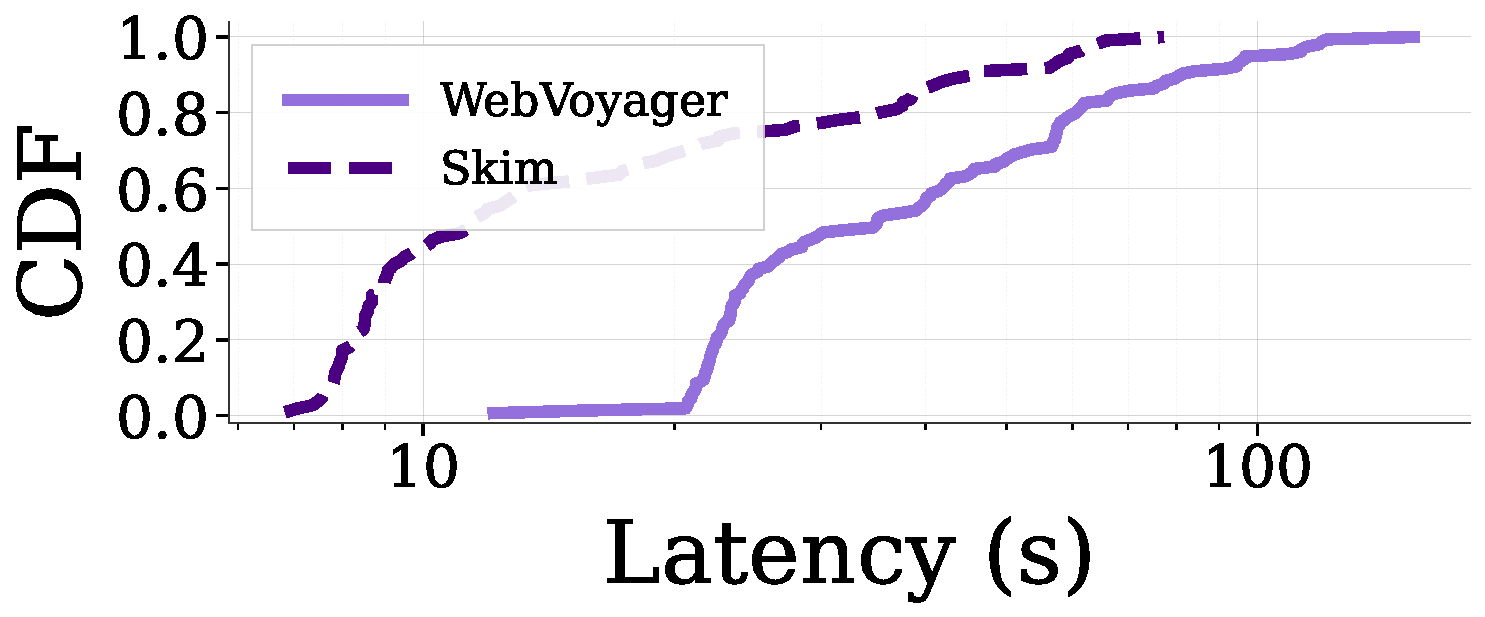
\includegraphics[width=\linewidth]{figures/latency_successful_tasks_webvoyager_evaluation_cdf.pdf}
    \end{minipage}
    \hfill
    \begin{minipage}{0.32\textwidth}
        \centering
        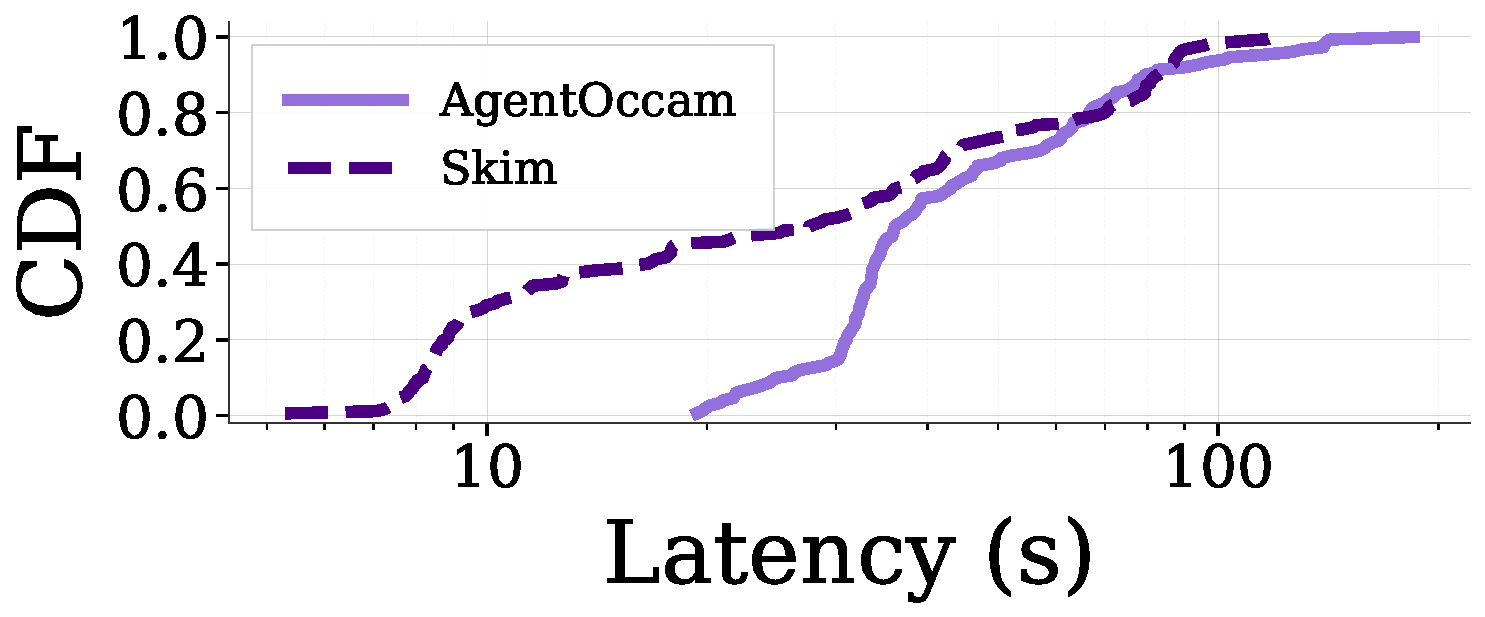
\includegraphics[width=\linewidth]{figures/latency_successful_tasks_agentoccam_evaluation_cdf.pdf}
    \end{minipage}
    \hfill
    \begin{minipage}{0.32\textwidth}
        \centering
        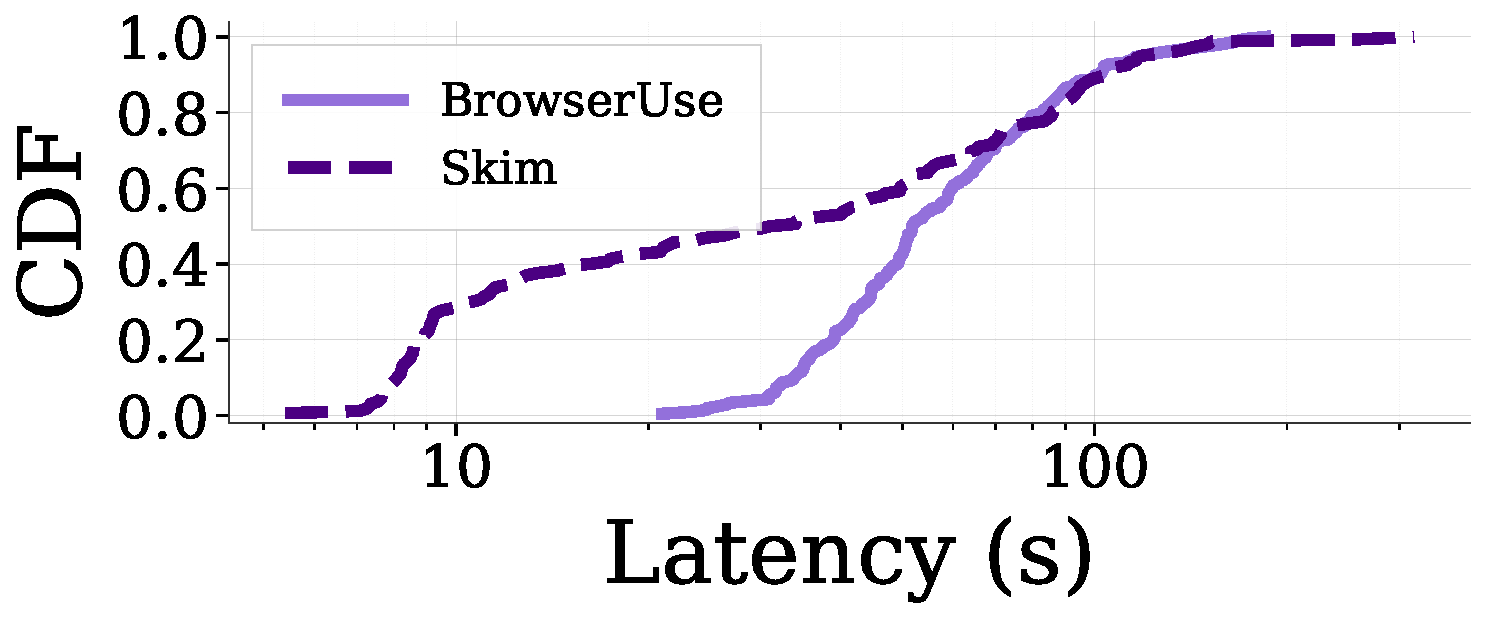
\includegraphics[width=\linewidth]{figures/latency_successful_tasks_browseruse_evaluation_cdf.pdf}
    \end{minipage}

    \tightcaption{End-to-end task latencies for WebVoyager (left), AgentOccam (middle), and BrowserUse (right) across all tasks.}
    \label{fig:end-to-end-latencies}
\end{figure*}
\begin{figure*}[t]
    \centering

    \begin{minipage}{0.32\textwidth}
        \centering
        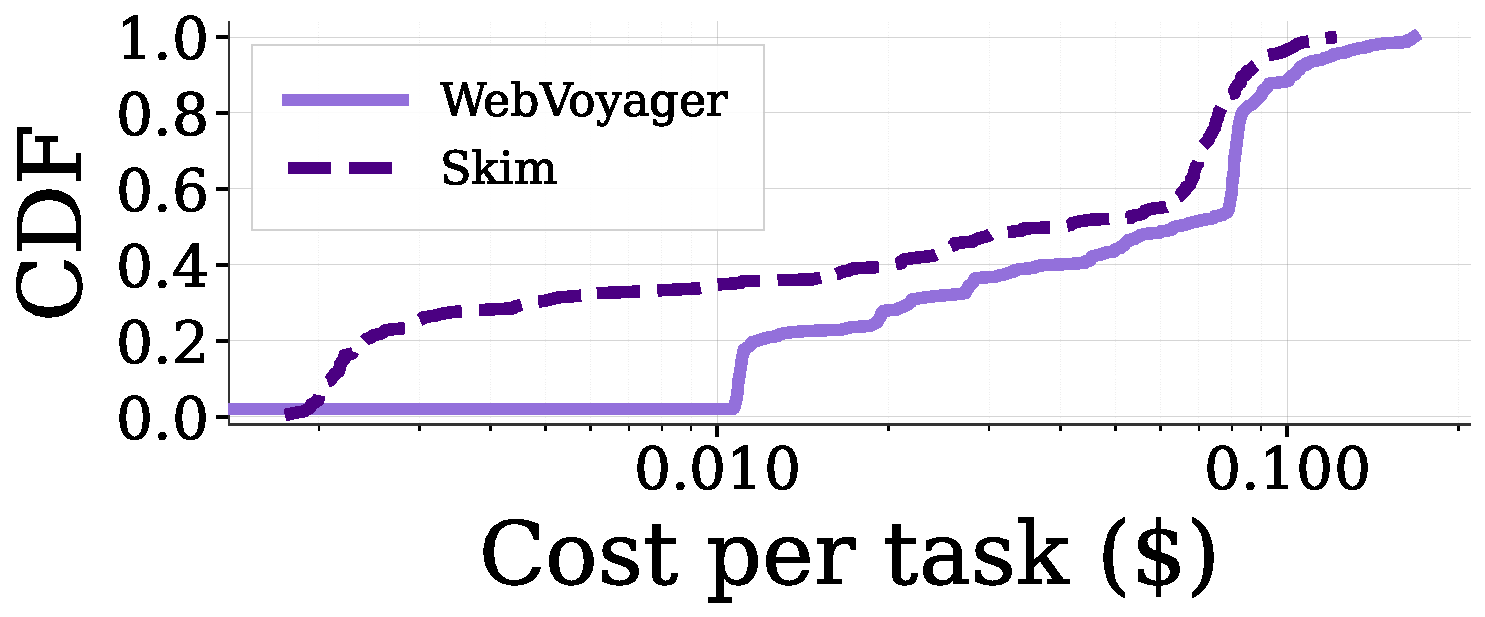
\includegraphics[width=\linewidth]{figures/monetary_costs_webvoyager_evaluation_cdf.pdf}
    \end{minipage}
    \hfill
    \begin{minipage}{0.32\textwidth}
        \centering
        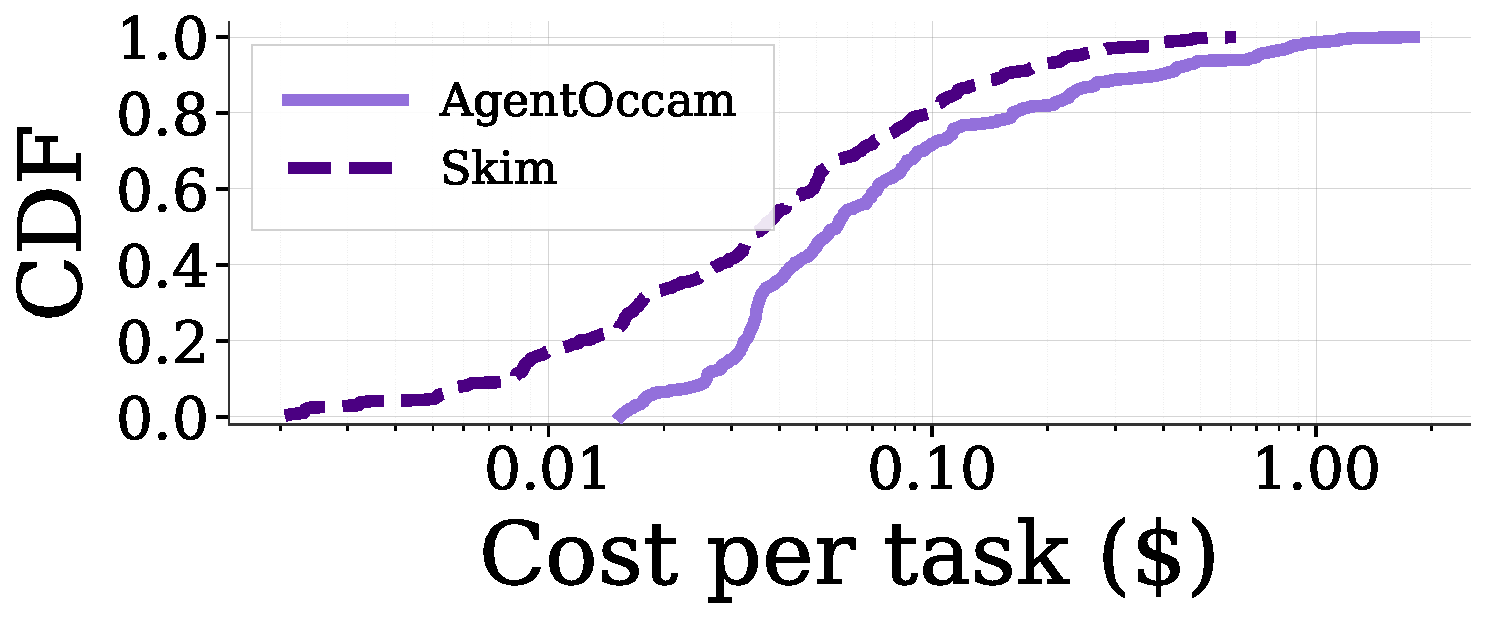
\includegraphics[width=\linewidth]{figures/monetary_costs_agentoccam_evaluation_cdf.pdf}
    \end{minipage}
    \hfill
    \begin{minipage}{0.32\textwidth}
        \centering
        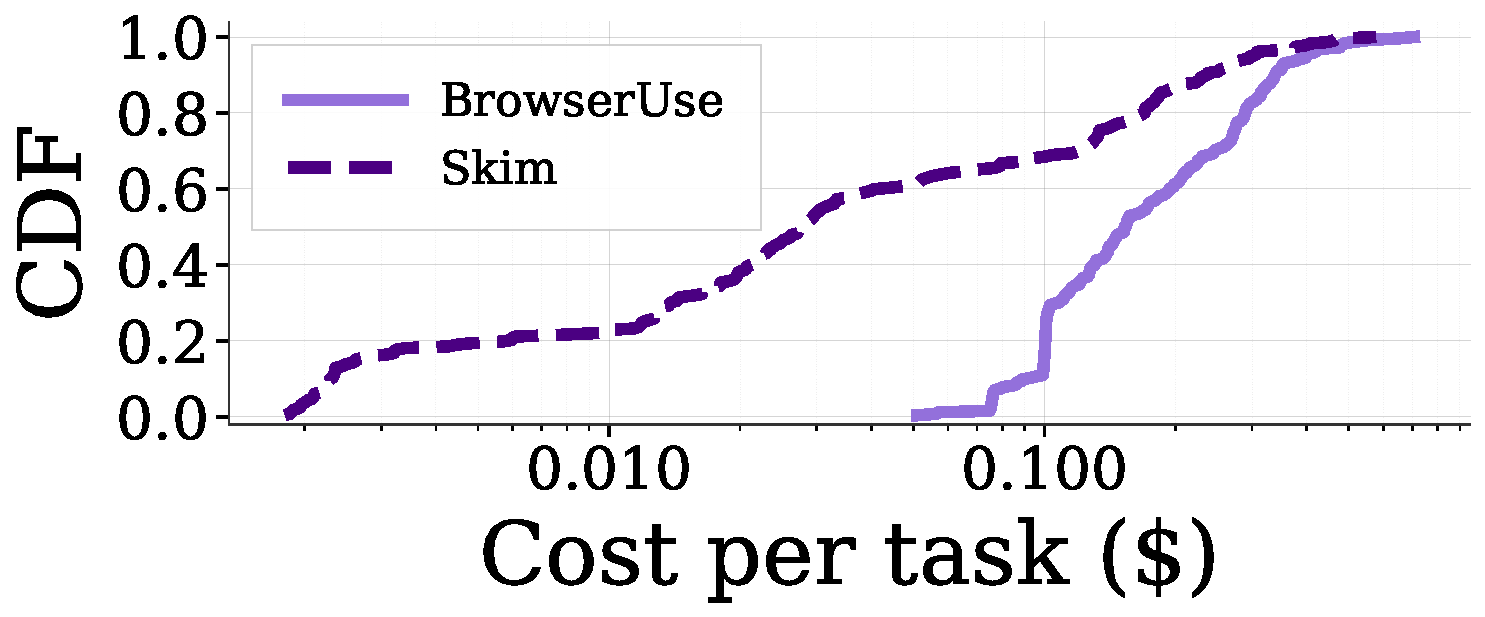
\includegraphics[width=\linewidth]{figures/monetary_costs_browseruse_evaluation_cdf.pdf}
    \end{minipage}

    \tightcaption{End-to-end task costs for WebVoyager (left), AgentOccam (middle), and BrowserUse (right) across all tasks.}
    \label{fig:end-to-end-costs}
\end{figure*}



\subsection{Methodology}
\begin{sloppypar}
We evaluate \sys atop three representative ReAct-based web agents: WebVoyager~\cite{webvoyager}, AgentOccam~\cite{agentoccam}, and BrowserUse~\cite{browseruse}. WebVoyager is a multimodal agent over rendered screenshots, serving as a strong baseline for general-purpose live-web navigation. AgentOccam emphasizes lightweight reasoning and action efficiency through aggressive state pruning over text-based DOM observations, representing cost-conscious agent designs. BrowserUse is a production-oriented browser-automation framework that tightly couples LLM reasoning with browser-control primitives, reflecting the deployment-focused agents used in retrieval and automation pipelines. Together, these systems span a range of reasoning styles, observation modalities, and execution overheads.
\end{sloppypar}

We consider two representative benchmarks. WebVoyager~\cite{webvoyager} spans 15 real-world websites with open-ended navigation, retrieval, and structured extraction tasks. WebShop~\cite{webshop} provides a shopping environment derived from Amazon product data, focused on multi-step product search and selection. Because evaluating live ReAct agents at scale is both computationally expensive and time-consuming (browsers and frontier models at each step), we conduct our experiments on a representative subset of 300+ tasks randomly drawn across the two benchmarks. Each task is executed on every agent backend with \sys. This scale captures a broad range of websites, task structures, and execution behaviors while keeping evaluation practically tractable. Ablations and detailed analyses are reported on AgentOccam and WebVoyager, though all trends hold for other combinations. Metrics include end-to-end latency, per-task dollar cost, and task success rate. Latency and cost are measured over complete task executions including failures and cascades.

%We evaluate \sys atop three representative ReAct-based web agents: WebVoyager, AgentOccam, and BrowserUse. WebVoyager is a canonical multimodal ReAct agent that operates over rendered webpages using iterative reasoning and browser interaction, and serves as a strong baseline for general-purpose live-web navigation. AgentOccam emphasizes lightweight reasoning and action efficiency through aggressive state pruning and simplified decision making, making it representative of cost-conscious agent designs. BrowserUse is a production-oriented browser automation framework that tightly couples LLM reasoning with browser control primitives and realistic interaction APIs, reflecting the growing class of deployment-focused web agents used in retrieval and automation pipelines. Together, these systems span a range of reasoning styles, observation modalities, and execution overheads, allowing us to evaluate whether \sys generalizes across diverse ReAct implementations rather than overfitting to a single agent architecture.


%We evaluate on two representative benchmarks: WebVoyager and WebShop. WebVoyager consists of live-web tasks spanning 15 real-world websites and exercises open-ended navigation, retrieval, and structured extraction. WebShop provides a controlled shopping environment derived from Amazon product data and focuses on multi-step product search and selection tasks. Because evaluating live ReAct agents is both computationally expensive and time-consuming (particularly in their default form using browsers and frontier models at each step), we conduct our experiments on a representative subset of 300 tasks randomly drawn across the two benchmarks. This scale is sufficient to capture a broad range of websites, task structures, and execution behaviors while keeping evaluation practically tractable.

%Metrics include end-to-end wall-clock latency, inclusive of routing, fetching, parsing, inference, verification, and cascade overhead; per-task dollar cost, including frontier API usage and local-model inference cost; and task success rate. Latency and cost are measured over complete task executions including failures and cascades.


% Ours webshop WebVoyager: 66 / 150, default: 72 / 151
% Ours WebVoyager WebVoyager 39 / 151 (upto20: 120 / 303), default: 41 / 150
%
% Ours webshop AgentOccam 83 / 150, default: 75 / 150
% Ours WebVoyager AgentOccam 73 / 151, default: 74 / 151
%
% Ours webshop browseruse 58 / 150, default: 71 / 150
% Ours WebVoyager browseruse 79 / 151, default: 64 / 151



\subsection{Main Results}

Figures~\ref{fig:end-to-end-latencies}-\ref{fig:end-to-end-costs} report per-task latency and cost CDFs against each baseline. \sys achieves its largest gains on tasks that complete on the speculative fast path: navigation collapses to direct URL synthesis, repeated frontier-model inference is avoided, and extraction runs over condensed HTML with lightweight models. These tasks complete at a small fraction of full-ReAct latency and cost. Gains diminish in the tail as tasks trigger fallback to the underlying ReAct agent, either because verification rejected the fast path or because no template matched. However, \sys often preserves partial navigational progress through warm-start URLs, so even fallbacks frequently outperform cold-start ReAct (Figures~\ref{fig:warm-start-webvoyager-savings}-\ref{fig:warm-start-agentoccam-savings}). At the far tail, performance converges to the baseline in two cases: when \sys determines that no fast path applies and routes directly to the ReAct backend, or when the speculative attempt reaches a URL without useful progress; for the latter, overhead is bound by the failed attempt and verification stage.

Despite the fallback cases, \sys preserves end-to-end accuracy within noise of full ReAct (Table~\ref{t:accuracy-comparison}) while substantially reducing median latency and cost. Two properties drive this. First, speculative execution follows trajectories grounded in real structural patterns from offline profiling -- URL templates, search behavior, pagination structure, answer schemas -- that are tied to the site's core purpose and remain stable even as underlying content changes, rather than unconstrained lightweight reasoning over arbitrary pages. Second, every fast-path result is gated through verification before commitment, catching missing fields, unexpected page structures, failed extraction, and stale templates. When verification rejects, \sys reverts to the full ReAct agent rather than committing a wrong answer, so failures degrade gracefully into standard agent behavior.
\begin{table}[t]
    \centering
    \small
    \begin{tabular}{lcc}
        \toprule
        \textbf{Agent} & \textbf{Our accuracy} & \textbf{Agent accuracy} \\
        \midrule
        WebVoyager & 40.6\% & 37.6\% \\
        AgentOccam & 52.0\% & 49.6\% \\
        BrowserUse & 45.6\% & 45.0\% \\
        \bottomrule
    \end{tabular}
    \vspace{8pt}
    \tightcaption{Accuracies for \sys and default web agents.}
        \label{t:accuracy-comparison}
\end{table}

\para{Aggregate mode.} \sys{}'s cost savings can be repurposed to run multiple speculative trials per task within the baseline's single-execution budget, with results aggregated across trajectories. For instance, on the WebVoyager benchmark with AgentOccam, this enables \sys to run an average of four additional trajectories per task, with accuracy wins varying by sampling strategy: upper-bound wins (i.e., assuming oracle selection of the best trial) reach 16.7 percentage points, while majority vote yields 4.2-percentage-point improvements. 



%On 24 tasks with five trials each, individual trials match baseline accuracy (19-21/24 per trial vs. 19/24 baseline), but aggregating lifts performance substantially: 23/24 tasks have at least one correct trial, and majority voting (≥3/5 correct) achieves 20/24. This translates to accuracy improvements of 4.2 percentage points (majority vote, 79.2\% → 83.3\%) and 16.7 percentage points (≥1 correct, 79.2\% → 95.8\%) over the baseline. The gain comes from \sys{}'s cost headroom enabling multiple trajectory explorations per task — a regime the baseline cannot afford — with verifier-based selection across trials.


\begin{comment}
Figures~\ref{fig:eval-latency-agentoccam} and
\ref{fig:eval-latency-webvoyager} report per-task latency CDFs
against each baseline. \sys achieves its largest gains on tasks
that successfully complete on the speculative fast path. In these
cases, the system bypasses the iterative ReAct loop entirely:
navigation collapses to direct URL synthesis and retrieval,
execution avoids repeated frontier-model inference, and extraction
runs over condensed HTML using lightweight models. These tasks
therefore complete with only a small fraction of the latency and
cost of full ReAct execution.

The gains diminish in the tail of the distribution as more tasks
trigger fallback to the underlying ReAct agent. Fallbacks occur
when verification rejects the speculative execution path or when
a task does not match a reusable template. Even in these cases,
however, \sys often preserves partial navigational progress through
warm-start URLs inherited from the failed fast path. As a result,
many fallback tasks still outperform cold-start ReAct execution
despite requiring full-agent recovery.

At the far tail, performance converges toward the baseline ReAct
agent. This occurs in two common cases: either \sys determines
ex ante that no reliable fast path applies and routes directly to
the ReAct backend, or the speculative trajectory reaches a URL
that provides little useful navigational progress, making recovery
behavior similar to executing the ReAct agent from scratch. In
the latter case, the additional overhead is limited to the small
cost of the failed speculative attempt and verification stage.
Importantly, despite these fallback cases, \sys preserves end-to-end
accuracy statistically within noise of full ReAct
(Figures~\ref{fig:eval-acc-webvoyager},
\ref{fig:eval-acc-webshop}) while substantially reducing median
latency and cost.

Against the capability-stripped baselines, \sys preserves the
coverage and robustness of full ReAct execution while approaching
the cost profile of lightweight retrieval pipelines on fast-path
tasks. The key reason accuracy is preserved is that speculative
execution is not based on heuristic shortcuts or approximate
trajectory guessing; it is grounded in real structural patterns
observed during offline profiling of each site. The fast path
reuses stable site conventions --- URL templates, search behavior,
pagination structure, and answer schemas --- that are tied to the
site’s core purpose and therefore remain comparatively stable over
time even as underlying content changes. As a result, speculative
execution follows trajectories that are already known to be valid
for that site rather than attempting unconstrained lightweight
reasoning over arbitrary pages.

Robust verification further prevents speculative errors from
propagating into incorrect final outputs. Every fast-path result is
validated through schema checks, content-consistency verification,
and runtime monitoring before commitment. When verification detects
that the speculative execution path may have diverged from the
task -- due to missing fields, unexpected page structure, failed
content extraction, or stale templates -- \sys automatically
reverts to the default ReAct agent. Because ReAct execution serves
as the recovery path rather than being replaced entirely, failures
of speculative execution degrade gracefully into standard agent
behavior instead of causing catastrophic task failure. In effect,
\sys preserves the accuracy envelope of full ReAct execution while
speculatively bypassing its cost whenever the site structure makes
doing so safe.
\end{comment}



\begin{figure}[t]
    \centering
    \begin{minipage}{0.48\columnwidth}
        \centering
        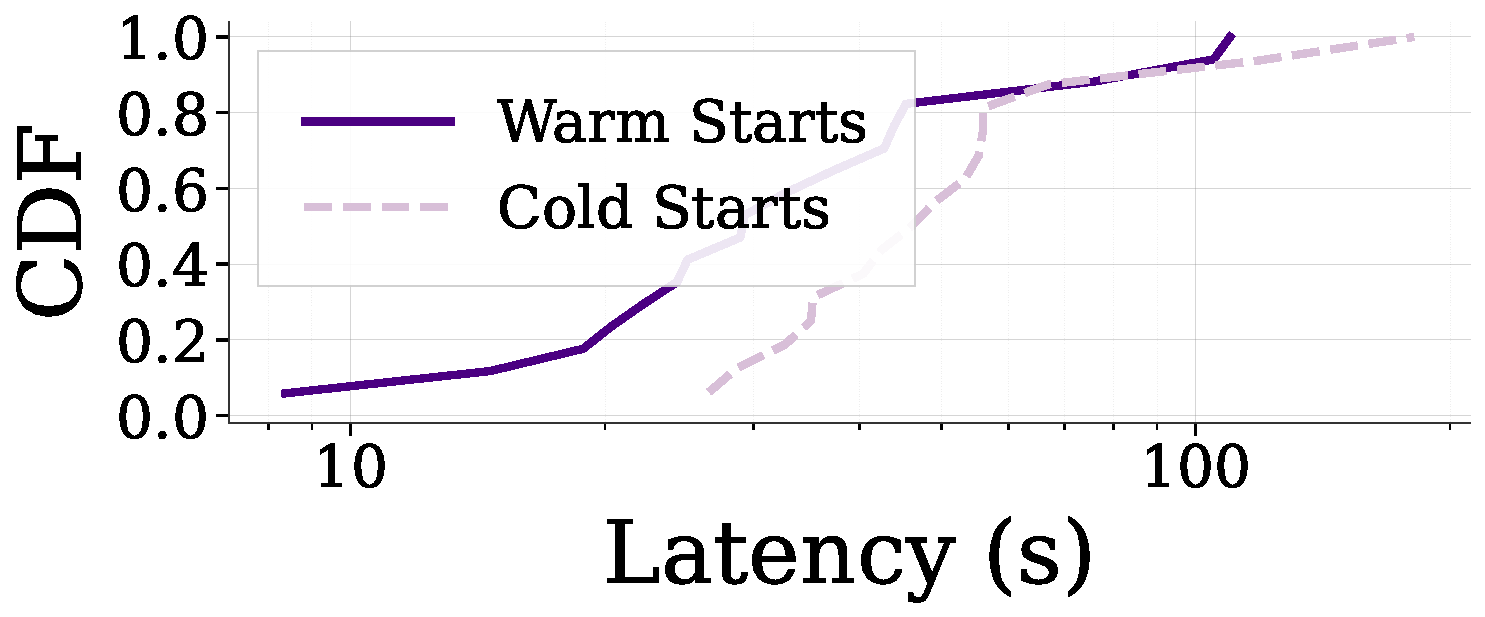
\includegraphics[width=\linewidth]{figures/latency_webvoyager_warm_cold_cdf.pdf}
        \tightcaption{Warm start savings for WebVoyager.}
        \label{fig:warm-start-webvoyager-savings}
    \end{minipage}
    \hfill
    \begin{minipage}{0.48\columnwidth}
        \centering
        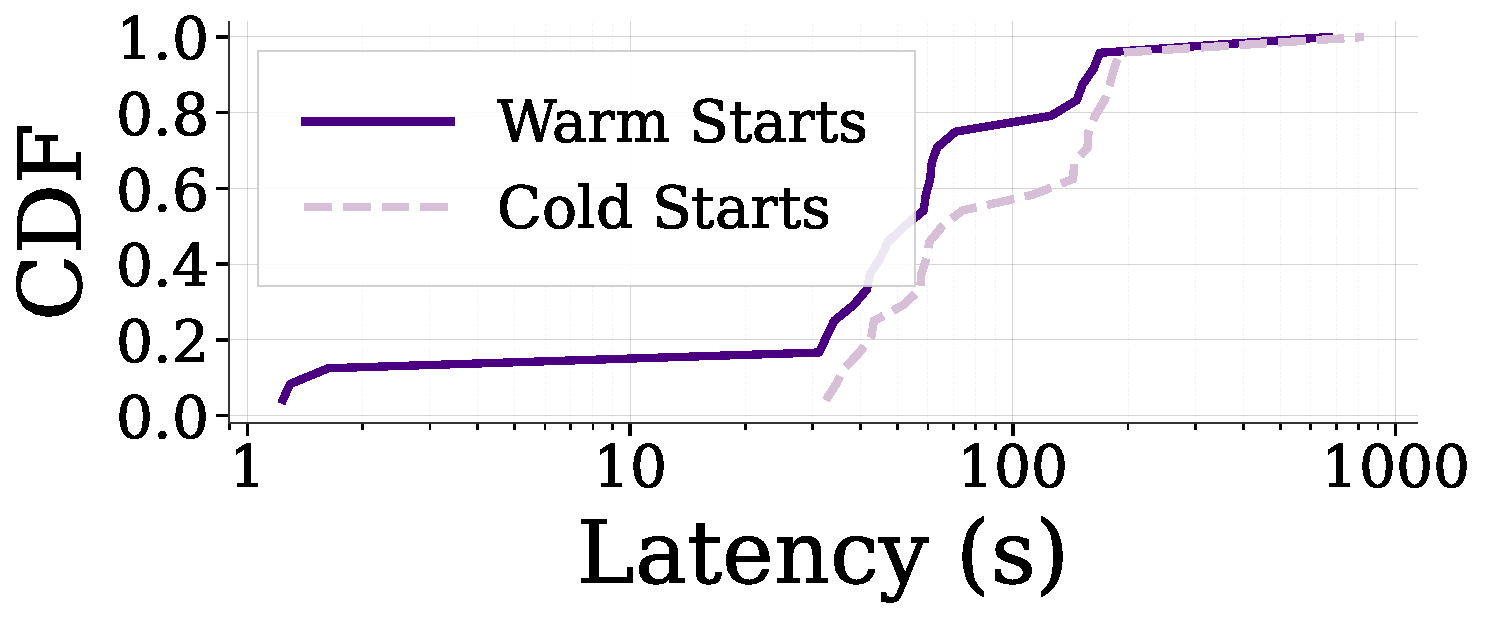
\includegraphics[width=\linewidth]{figures/latency_agentoccam_warm_cold_cdf.pdf}
        \tightcaption{Warm start savings for AgentOccam.}
        \label{fig:warm-start-agentoccam-savings}
    \end{minipage}
\end{figure}


% Results we want to get: latency of fast path vs default, Accuracy of fast path vs default
% Latencies and costs by task

\begin{figure}[t]
    \centering
    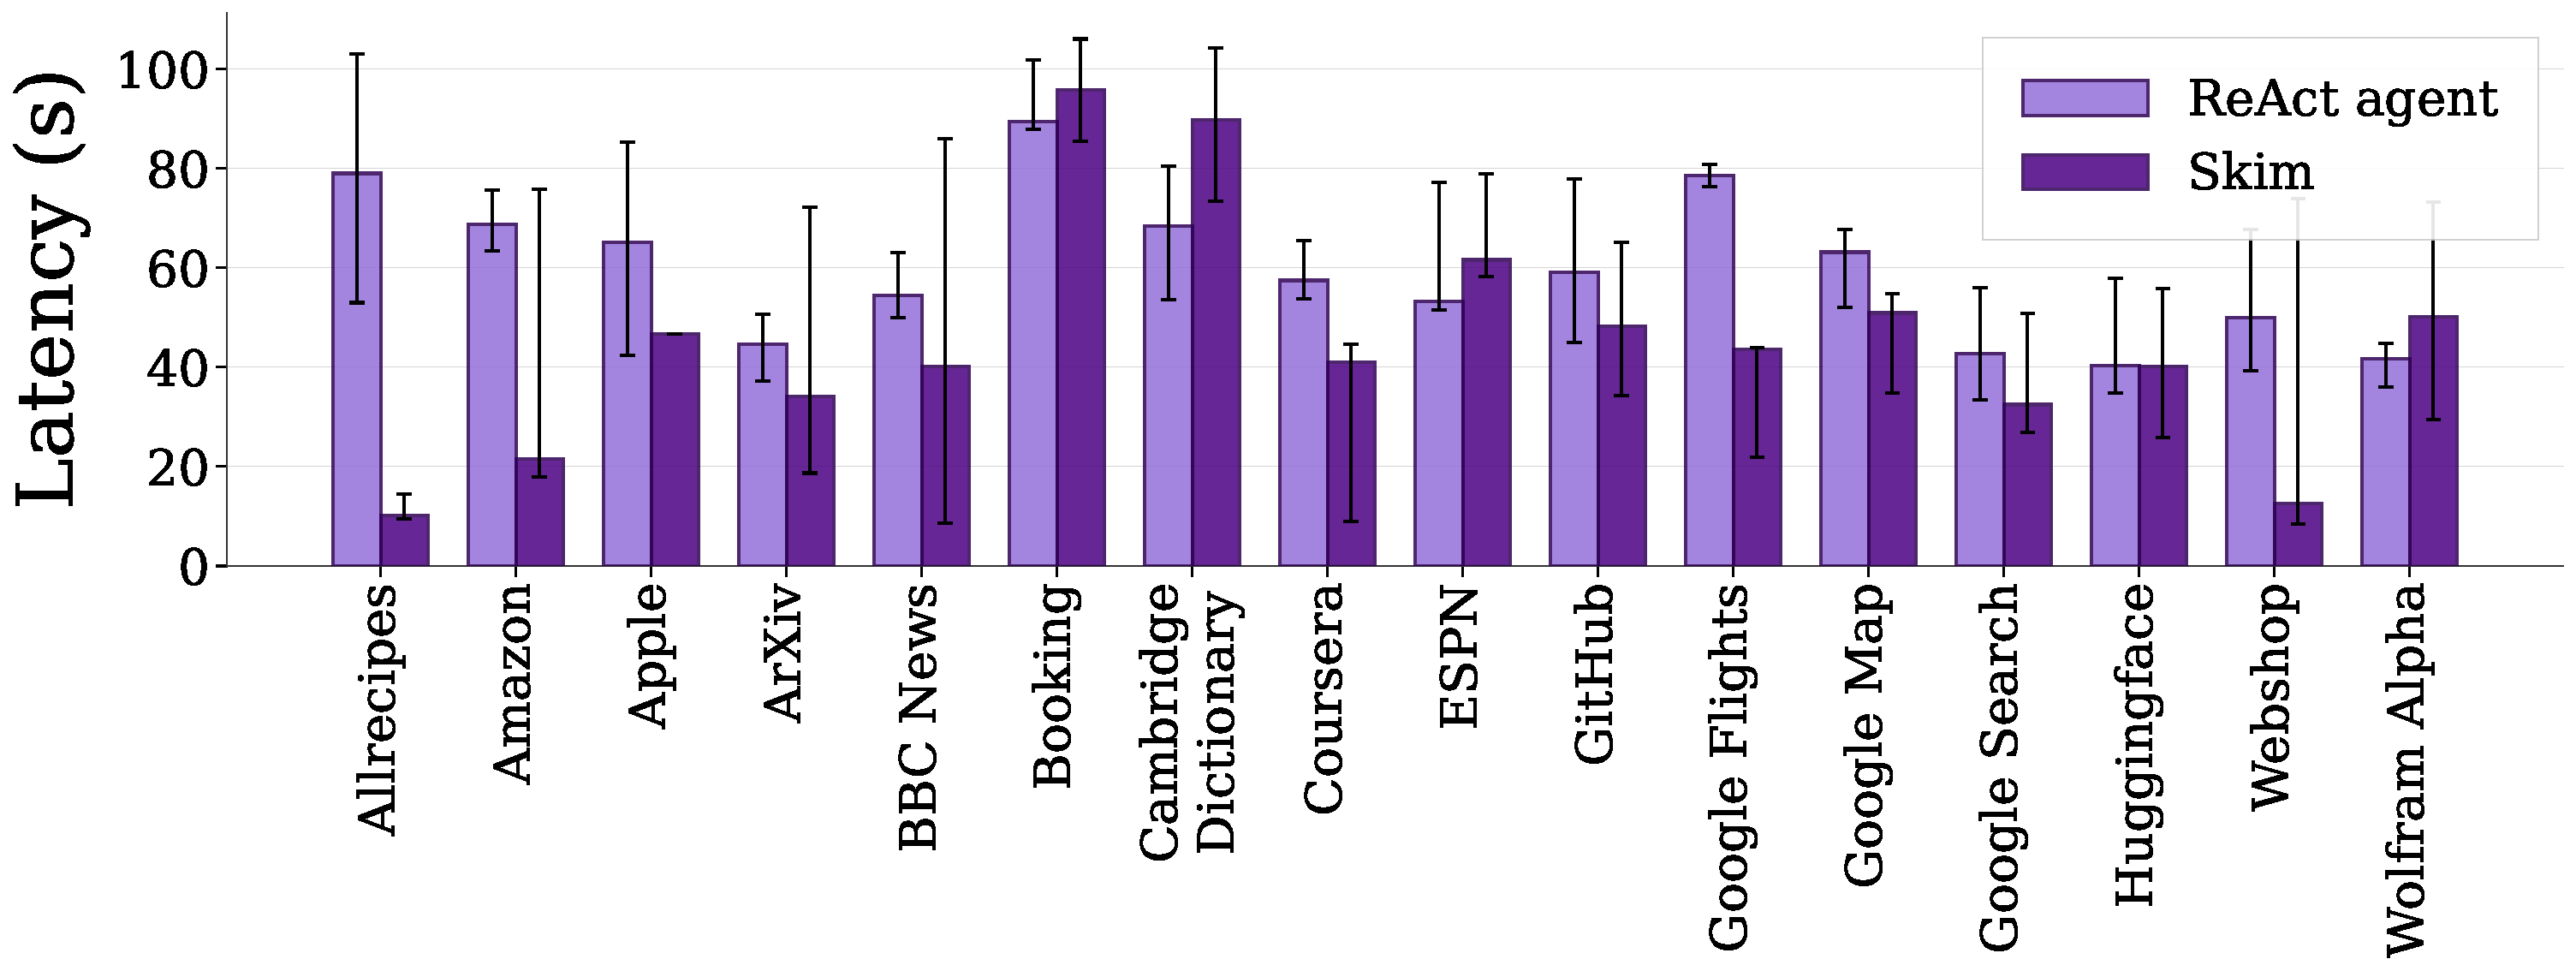
\includegraphics[width=0.9\columnwidth]{figures/latency_successful_breakdown_by_task_cdf.pdf}
    \tightcaption{Median end-to-end latency by website; error bars show 25th/75th percentiles. }
    \label{fig:eval-latency-breakdown-by-task}
\end{figure}

\para{Per-site speedups.}
Figure~\ref{fig:eval-latency-breakdown-by-task} reports median end-to-end latency across websites with heterogeneous retrieval and interaction structure. \sys{} achieves the largest speedups on sites whose workflows are dominated by structured search, filtering, and retrieval over stable page schemas. In these settings, speculative execution collapses multi-step browser interaction into direct URL synthesis followed by lightweight extraction over cleaned HTML, bypassing most of the iterative ReAct loop and avoiding many sequential browser actions and frontier-model inference calls. These gains are not tied to any single benchmark or domain; they emerge whenever a site exposes reusable navigation conventions and answer-bearing content resolvable through direct retrieval.

Latency improvements diminish on sites where speculation more frequently triggers fallback. These cases generally arise when site structure is difficult to parameterize through stable templates alone -- heavily JavaScript-driven interfaces, aggressive bot-detection, multimodal content requiring visual reasoning, or search semantics highly sensitive to exact query phrasing -- making direct retrieval less reliable and increasing verification failure and cascade. A small number of tasks also show speculative execution slightly increasing latency relative to the baseline, primarily when the warm start provides little useful navigational progress or when nondeterminism in LLM-based agent execution causes the baseline agent to converge unusually quickly. Even then, the overhead from failed speculation remains small relative to the cost of full browser-agent execution.

\para{Decomposing the savings gap.}
Two structural factors gap our savings from the hand-engineered ceiling. First, \sys pays a generalization tax of ~5-6s per task for routing, URL synthesis, and capability prediction. Second, only 12.6-45.3\% complete on the fast path; the rest cascade with warm-started ReAct, which captures most of the remaining gain through prefix-sharing rather than direct speculation success.
\begin{figure}[t]
    \centering
    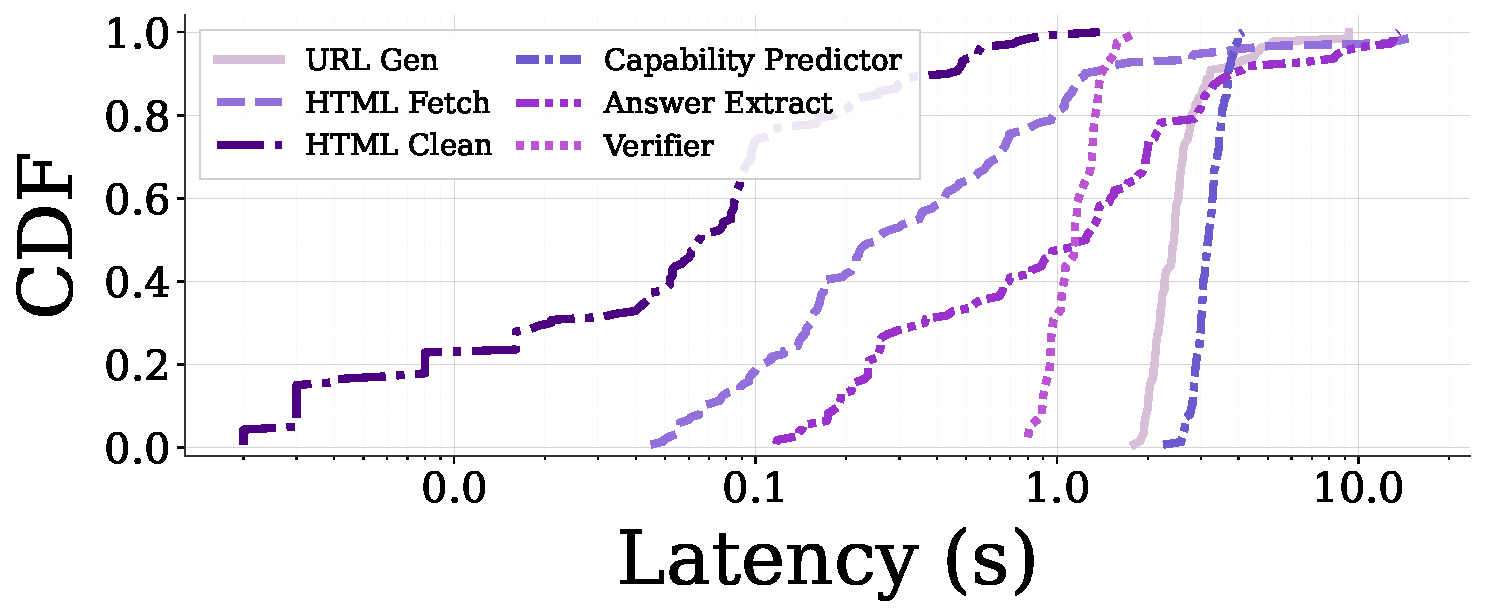
\includegraphics[width=0.9\columnwidth]{figures/ours_component_breakdown.pdf}
    \tightcaption{Per-task latency breakdown}
    \label{fig:eval-latency-breakdown}
\end{figure}

\para{Impact of warm starts.}
Figures~\ref{fig:warm-start-webvoyager-savings} and
\ref{fig:warm-start-agentoccam-savings} compare fallback latency
under warm- vs cold-started ReAct execution. Warm starts reduce fallback latency by
seeding the downstream agent with the URL reached during
speculative execution instead of restarting from the homepage.
Even when the fast path fails, it often resolves substantial
parts of the trajectory (search, filtering, pagination, query
construction), so fallback resembles local recovery from a
near-correct state rather than exploratory browsing from
scratch. The latency distributions show that this substantially
compresses the tail of expensive fallback trajectories across
both agents. This reflects the prefix-sharing property:
incorrect speculative trajectories remain close enough to the
correct path that ReAct recovers with little additional
exploration, allowing \sys{} to preserve latency gains even on
cascade.


\subsection{Detailed Analysis}

\para{Latency breakdown.}
We decompose per-task latency across system components to identify where time is spent along the speculative execution path. Figure~\ref{fig:eval-latency-breakdown} reports stage-level wall-clock latency for fast-path-completing tasks across six stages: routing and capability prediction, URL synthesis, HTTP fetch, HTML cleaning, lightweight extraction, and verification. The dominant costs arise not from web access itself, but from the lightweight semantic stages responsible for interpreting and parameterizing tasks: routing and capability prediction take $\sim$3s per task, and URL synthesis another $\sim$2--3s for most queries (with a small long tail reaching $\sim$9s). By contrast, the systems-oriented stages are extremely cheap: HTTP fetches typically complete within 100--300ms, and HTML cleaning is usually below 100ms. This highlights a central property of read-only web tasks: once the correct destination URL is known, retrieving and condensing the relevant content is inexpensive relative to discovering that URL through exploratory browser interaction.

Extraction latency exhibits the largest variance: simple schema-constrained retrievals complete in well under a second, while harder synthesis-style tasks occasionally require 8--14s of local-model reasoning. Verification adds only $\sim$1s of overhead, preserving the design goal that correctness checking remain cheaper than the speculative execution it validates. For cascaded tasks, the full ReAct loop dominates tail latency, but failed fast paths frequently still preserve useful navigational progress through warm-start URLs, allowing the downstream agent to resume near the relevant destination page rather than restarting from the homepage. Per-task cost follows the same asymmetry: fast-path tasks are dominated by inexpensive local-model inference and HTTP execution, while cascaded tasks inherit the frontier-model cost profile of full browser-agent execution.

\begin{figure}[t]
    \centering
    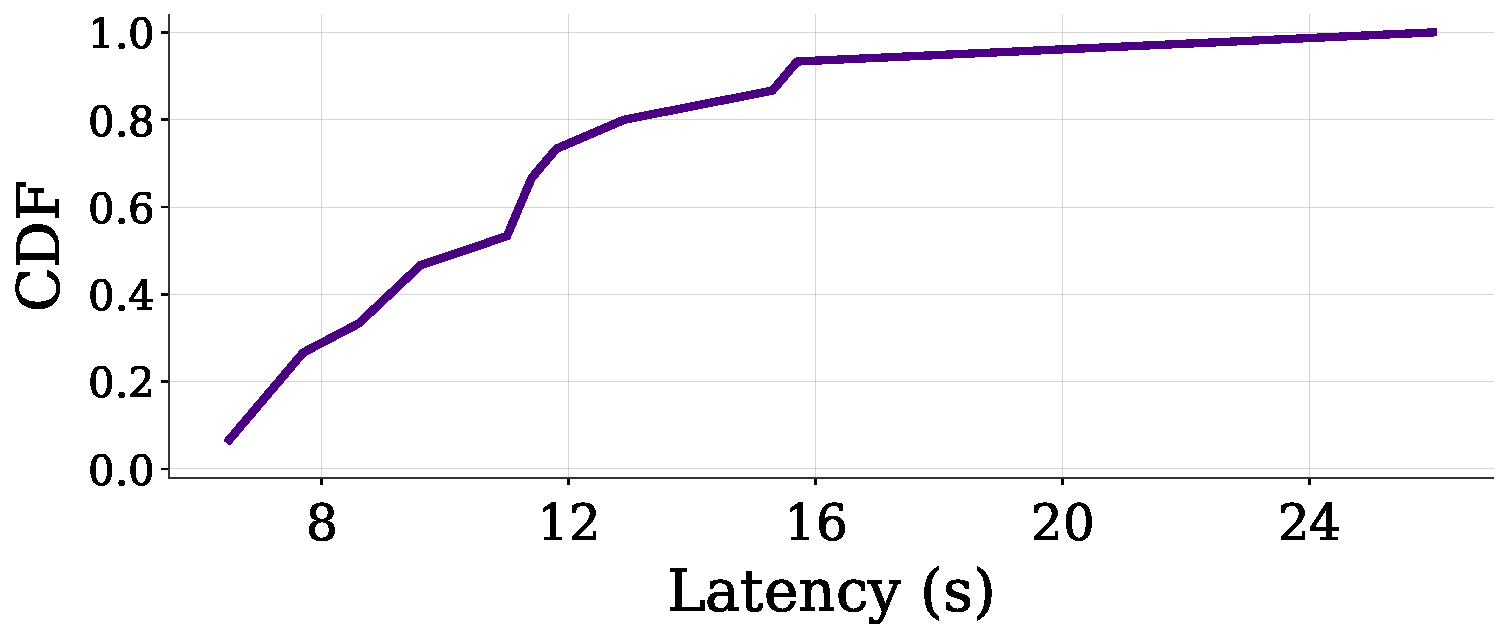
\includegraphics[width=0.9\columnwidth]{figures/offline_probing_latencies_cdf.pdf}
    \tightcaption{Offline profiling latency per site. }
    \label{fig:offline-profiling-cdf}
\end{figure}


\para{Verification cost vs. quality.} The verifier must satisfy two goals: it must remain cheap enough that verification does not erase the fast path's savings, while being conservative enough that incorrect speculative answers rarely commit. We therefore explicitly bias the verifier toward rejection and aggressive cascade rather than risking false accepts: borderline or weakly-supported speculative outputs are escalated to heavier execution tiers instead of being committed directly.

We compare \sys's lightweight verifier against a frontier-model verifier that scores candidate answers against the full DOM. The lightweight verifier is 11.5$\times$ cheaper per call while achieving 82.0\% precision and 86.2\% recall (F1 = 0.84, accuracy = 86.9\%). Reliability is highest on sites with structured, schema-friendly outputs and lower on sites with heavier client-side rendering or looser semantics; importantly, these are also the sites where speculative execution more frequently triggers fallback, so verifier uncertainty naturally translates into cascade rather than silently committed errors.

\para{Offline profiling pipeline.}
Figure~\ref{fig:offline-profiling-cdf} shows the one-time cost
of offline profiling. Profiling completes within 10s for
${\sim}40$\% of sites and within 12s for ${\sim}60$\%, with a
small tail toward 16s on structurally complex sites requiring
browser escalation, dynamic rendering, or bot-detection
handling. The cost stays this low because the profiler captures
the small set of URL templates and answer schemas that cover
common-case tasks rather than enumerating every page or query
the site supports; tasks that fall outside profiled patterns
are detected at match time and routed to the ReAct fallback, so
coverage gaps cost nothing in correctness. The cost is amortized
across all future tasks on the site and does not contribute to
online query latency. Profiles are continuously validated
through schema and content-consistency checks at runtime; stale
profiles are regenerated when structural drift is detected.



% \para{Comparison with stateless retrieval pipelines.}
% Production retrieval-augmented assistants (Perplexity, Gemini
% grounded search, ChatGPT browsing) operate as stateless retrieval
% pipelines: they issue a query to a search API, fetch the top-ranked
% results, and synthesize an answer. This pattern is efficient on
% tasks whose answers are surfaced by search-engine indices but is
% structurally bounded by index coverage. Our SearXNG+GPT-4o baseline,
% a representative single-shot instance of this pattern, succeeds on
% $S_{sr}$\% of WebVoyager tasks at \$$C_{sr}$ per task. It fails on
% the regime stateless retrieval is structurally limited on:
% authenticated or session-bound pages, multi-step trajectories whose
% intermediate states are not search-indexed, and freshly-published
% or niche content beyond search-engine coverage. \sys reaches
% stateless-retrieval cost on its fast path while preserving full
% ReAct's coverage on the cascaded tail, occupying a different point
% in the cost-coverage tradeoff than either pure approach. \todo{Need to get these stateless retrieval numbers}




% \section{Related Work}
% \label{sec:related}

% To our knowledge, \sys is the first system to treat website structure as a speculative execution primitive for accelerating general-purpose web agents. Prior work instead improves agent policies and web-agent benchmarks, accelerates inference or agent execution, or exploits webpage structure for extraction and pruning. We discuss these lines of related work below.


% \para{Web agents and benchmarks.}
% Recent work has rapidly expanded both the scope of LLM-based web agents and the realism of their evaluation environments. Early systems such as WebGPT~\cite{webgpt} and ReAct~\cite{react} established the paradigm of interleaving reasoning with actions over external environments, with subsequent work improving planning, observation representations, grounding, prompting, program synthesis, skill reuse, and benchmark realism~\cite{webagent,mind2web,webshop,webarena,weblinx,webvoyager,gaia,odysseys,webxskill,seeact,agentoccam,molmoweb,browseruse}, alongside interface perception and grounding work that improves how agents observe and act on interfaces~\cite{showui,uground,pixels2uiactions}. The closest antecedent is WebAgent~\cite{webagent}, which pushes execution in a more programmatic direction through planning, understanding, and program synthesis to generate executable scripts for real websites rather than one-step-at-a-time action selection. Its motivation is adjacent to ours, but the core question differs: WebAgent improves the agent policy and execution strategy inside the online loop, whereas \sys asks when that loop can be bypassed altogether through a verified site-structured fast path. More broadly, prior systems strengthen the policy or evaluation setting of the underlying agent but still execute a largely uniform browser-and-LLM loop online; \sys instead targets the execution substrate beneath those agents, speculating away repeated browser and frontier-model use when site structure makes a cheaper path safe.

% \para{Speculation, cascades, and efficient LLM serving.}
% Another line of work targets efficiency through multi-model routing, token-level speculation, and speculative execution inside agent loops. FrugalGPT~\cite{frugalgpt} learns cascades over models to reduce per-query cost, while most speculation work targets wall-clock latency: speculative decoding accelerates generation by drafting with a smaller model and verifying with a larger one~\cite{speculative_decoding}, and related agent-side techniques add auxiliary drafting, branching, or verification work to shorten response time~\cite{contextbudget,readmorethinkmore,dsp,speculative_actions,speccache}. These methods reduce latency but often by spending extra compute, sometimes substantially increasing monetary cost. \sys shares the intuition that cheap predictions can be validated before paying for a stronger execution path, but applies it at a different granularity and objective: our speculation is over \emph{site-structured fast paths and execution tiers} rather than tokens, cached environment responses, compressed context alone, or next actions inside an unchanged agent loop. We speculate on direct URLs, HTTP-only execution, and schema-constrained extraction, falling back to the full web agent only when verification fails. As a result, \sys reduces latency and monetary cost simultaneously by removing browser work and entire ReAct steps, rather than adding speculative computation in front of the same underlying execution.

% \para{Wrapper induction and web extraction.}
% \sys also relates to classical wrapper induction for semi-structured web pages, which exploits the regularity of site templates to extract data reliably and efficiently~\cite{kushmerick2000wrapper}. Modern web-agent work revisits similar questions through HTML-specific modeling, structured DOM reasoning, DOM pruning, region-level observation abstractions, and explicit executable skill artifacts~\cite{html_understanding,domqnet,prune4web,region4web,contractskill}. \sys operates one level earlier: instead of compressing the page after the agent reaches it, it uses site structure to predict when the browser and much of the trajectory can be skipped entirely. This literature shares our core observation that purpose-built websites expose stable structure across many pages, but our setting is broader in two ways. First, we use site structure not only for extraction or DOM reduction but also for URL synthesis, retrieval-mode selection, and runtime verification. Second, wrapper-, abstraction-, and pruning-based systems were not designed to solve the full fast-path routing problem for general-purpose web agents: they do not address how to apply a speculative fast path aggressively enough to save browser and model cost while preserving end-to-end accuracy when the fast path is wrong. \sys thus uses wrapper-like structure as a speculative fast path rather than the only execution mode.
\section{Related Work}
\label{sec:related}

To our knowledge, \sys is the first system to treat website
structure as a speculative execution primitive for accelerating
web agents. Prior work instead improves agent
policies and benchmarks, accelerates inference and execution, or
exploits webpage structure for extraction and compression.

\para{Web agents and benchmarks.}
Recent work has rapidly expanded the capabilities of LLM-based
web agents and the realism of their evaluation environments.
Early systems such as WebGPT~\cite{webgpt} and
ReAct~\cite{react} established the paradigm of interleaving
reasoning with actions over external environments, with later
work improving planning, grounding, prompting, observation
representations, skill reuse, program synthesis, and benchmark
realism~\cite{webagent,mind2web,webshop,webarena,weblinx,webvoyager,gaia,odysseys,webxskill,seeact,agentoccam,molmoweb,browseruse},
alongside interface grounding and perception
work~\cite{showui,uground,pixels2uiactions}. The closest
antecedent is WebAgent~\cite{webagent}, which synthesizes
executable programs for websites.
Its motivation is adjacent to ours, but the core question
differs: WebAgent improves the policy operating inside the online
loop, whereas \sys asks when that loop can be bypassed entirely
through verified site-structured fast paths. More broadly, prior
systems strengthen the underlying agent but still execute a
mostly uniform browser-and-LLM loop online; \sys instead targets
the execution substrate itself, speculating away browser
interaction and frontier-model use when site structure makes a
cheaper path safe.

\para{Speculation and efficient inference.}
Another line of work targets efficiency through model cascades,
routing, and speculative execution. FrugalGPT~\cite{frugalgpt}
learns cascades over models to reduce cost, while speculative
decoding accelerates generation by drafting with a smaller model
and verifying with a larger one~\cite{speculative_decoding}.
Related approaches reduce latency through auxiliary drafting,
branching, caching, or verification
work~\cite{contextbudget,readmorethinkmore,dsp,speculative_actions,speccache}.
These methods operate primarily at the level of tokens, context,
or next-action prediction within an otherwise unchanged agent
loop. \sys instead speculates over \emph{site-structured
execution paths}: direct URLs, HTTP-only retrieval, and
schema-constrained extraction. Rather than adding speculative
computation ahead of the same browser trajectory, \sys removes
browser interaction and entire ReAct steps whenever verification
accepts the fast path.

\para{Wrapper induction and web extraction.}
\sys also relates to classical wrapper induction for
semi-structured webpages~\cite{kushmerick2000wrapper} and modern
work on HTML understanding, DOM reasoning, pruning, and
region-level abstractions~\cite{html_understanding,domqnet,prune4web,region4web,contractskill}.
These systems exploit recurring webpage structure for extraction
or observation compression \emph{after} the agent reaches the page.
\sys operates one level earlier: it uses site structure not only
for extraction, but also for URL synthesis, retrieval-mode
selection, speculative execution, and runtime verification. In
this sense, wrapper-like structure becomes a verified fast path
rather than the sole execution mode.
\section{Conclusion}

%This paper presented \sys, a speculative execution framework that accelerates web agents by exploiting per-site structural predictability. \sys captures stable site patterns in offline profiles, uses them at runtime to attempt cheap fast paths that bypass browsers and frontier models, and falls back to the full agent only when needed for accuracy. Across popular benchmarks and web agents, \sys reduces median per-task cost by 1.9$\times$ and latency by 33\% while preserving end-to-end accuracy.

We present \sys, a speculative execution framework that makes web agents substantially faster and cheaper without sacrificing the coverage of full ReAct execution. \sys exploits the structural regularity of purpose-built websites to replace much of the default browser-and-frontier-model loop with direct retrieval, lightweight extraction, and cheap verification, while preserving robustness through warm-started fallback when speculation fails. In accelerate mode, \sys reduces median per-task cost by 1.9$\times$ and latency by 33.4\% across three diverse ReAct backends while preserving end-to-end accuracy. In aggregate mode, the savings support an average of four additional speculative trials per task, improving accuracy by up to 16.7 percentage points (4.2 pp with majority vote). %Together, our results suggest that structure-aware speculation can make live-website agents more economically viable at large deployment scale.




\bibliographystyle{plain}
\bibliography{references}



% \clearpage
% \appendix
% \input{appendix}

\end{document}



